\documentclass{beamer}

% xcolor and define colors -------------------------
\usepackage{xcolor}

% https://www.viget.com/articles/color-contrast/
\definecolor{purple}{HTML}{5601A4}
\definecolor{navy}{HTML}{0D3D56}
\definecolor{ruby}{HTML}{9a2515}
\definecolor{alice}{HTML}{107895}
\definecolor{daisy}{HTML}{EBC944}
\definecolor{coral}{HTML}{F26D21}
\definecolor{kelly}{HTML}{829356}
\definecolor{cranberry}{HTML}{E64173}
\definecolor{jet}{HTML}{131516}
\definecolor{asher}{HTML}{555F61}
\definecolor{slate}{HTML}{314F4F}

% Mixtape Sessions
\definecolor{picton-blue}{HTML}{00b7ff}
\definecolor{violet-red}{HTML}{ff3881}
\definecolor{sun}{HTML}{ffaf18}
\definecolor{electric-violet}{HTML}{871EFF}

% Main theme colors
\definecolor{accent}{HTML}{00b7ff}
\definecolor{accent2}{HTML}{871EFF}
\definecolor{gray100}{HTML}{f3f4f6}
\definecolor{gray800}{HTML}{1F292D}


% Beamer Options -------------------------------------

% Background
\setbeamercolor{background canvas}{bg = white}

% Change text margins
\setbeamersize{text margin left = 15pt, text margin right = 15pt} 

% \alert
\setbeamercolor{alerted text}{fg = accent2}

% Frame title
\setbeamercolor{frametitle}{bg = white, fg = jet}
\setbeamercolor{framesubtitle}{bg = white, fg = accent}
\setbeamerfont{framesubtitle}{size = \small, shape = \itshape}

% Block
\setbeamercolor{block title}{fg = white, bg = accent2}
\setbeamercolor{block body}{fg = gray800, bg = gray100}

% Title page
\setbeamercolor{title}{fg = gray800}
\setbeamercolor{subtitle}{fg = accent}

%% Custom \maketitle and \titlepage
\setbeamertemplate{title page}
{
    %\begin{centering}
        \vspace{20mm}
        {\Large \usebeamerfont{title}\usebeamercolor[fg]{title}\inserttitle}\\
        {\large \itshape \usebeamerfont{subtitle}\usebeamercolor[fg]{subtitle}\insertsubtitle}\\ \vspace{10mm}
        {\insertauthor}\\
        {\color{asher}\small{\insertdate}}\\
    %\end{centering}
}

% Table of Contents
\setbeamercolor{section in toc}{fg = accent!70!jet}
\setbeamercolor{subsection in toc}{fg = jet}

% Button 
\setbeamercolor{button}{bg = accent}

% Remove navigation symbols
\setbeamertemplate{navigation symbols}{}

% Table and Figure captions
\setbeamercolor{caption}{fg=jet!70!white}
\setbeamercolor{caption name}{fg=jet}
\setbeamerfont{caption name}{shape = \itshape}

% Bullet points

%% Fix left-margins
\settowidth{\leftmargini}{\usebeamertemplate{itemize item}}
\addtolength{\leftmargini}{\labelsep}

%% enumerate item color
\setbeamercolor{enumerate item}{fg = accent}
\setbeamerfont{enumerate item}{size = \small}
\setbeamertemplate{enumerate item}{\insertenumlabel.}

%% itemize
\setbeamercolor{itemize item}{fg = accent!70!white}
\setbeamerfont{itemize item}{size = \small}
\setbeamertemplate{itemize item}[circle]

%% right arrow for subitems
\setbeamercolor{itemize subitem}{fg = accent!60!white}
\setbeamerfont{itemize subitem}{size = \small}
\setbeamertemplate{itemize subitem}{$\rightarrow$}

\setbeamertemplate{itemize subsubitem}[square]
\setbeamercolor{itemize subsubitem}{fg = jet}
\setbeamerfont{itemize subsubitem}{size = \small}







% Links ----------------------------------------------

\usepackage{hyperref}
\hypersetup{
  colorlinks = true,
  linkcolor = accent2,
  filecolor = accent2,
  urlcolor = accent2,
  citecolor = accent2,
}


% Line spacing --------------------------------------
\usepackage{setspace}
\setstretch{1.1}


% \begin{columns} -----------------------------------
\usepackage{multicol}


% Fonts ---------------------------------------------
% Beamer Option to use custom fonts
\usefonttheme{professionalfonts}

% \usepackage[utopia, smallerops, varg]{newtxmath}
% \usepackage{utopia}
\usepackage[sfdefault,light]{roboto}

% Small adjustments to text kerning
\usepackage{microtype}



% Remove annoying over-full box warnings -----------
\vfuzz2pt 
\hfuzz2pt


% Table of Contents with Sections
\setbeamerfont{myTOC}{series=\bfseries, size=\Large}
\AtBeginSection[]{
        \frame{
            \frametitle{Roadmap}
            \tableofcontents[current]   
        }
    }


% Tables -------------------------------------------
% Tables too big
% \begin{adjustbox}{width = 1.2\textwidth, center}
\usepackage{adjustbox}
\usepackage{array}
\usepackage{threeparttable, booktabs, adjustbox}
    
% Fix \input with tables
% \input fails when \\ is at end of external .tex file
\makeatletter
\let\input\@@input
\makeatother

% Tables too narrow
% \begin{tabularx}{\linewidth}{cols}
% col-types: X - center, L - left, R -right
% Relative scale: >{\hsize=.8\hsize}X/L/R
\usepackage{tabularx}
\newcolumntype{L}{>{\raggedright\arraybackslash}X}
\newcolumntype{R}{>{\raggedleft\arraybackslash}X}
\newcolumntype{C}{>{\centering\arraybackslash}X}

% Figures

% \imageframe{img_name} -----------------------------
% from https://github.com/mattjetwell/cousteau
\newcommand{\imageframe}[1]{%
    \begin{frame}[plain]
        \begin{tikzpicture}[remember picture, overlay]
            \node[at = (current page.center), xshift = 0cm] (cover) {%
                \includegraphics[keepaspectratio, width=\paperwidth, height=\paperheight]{#1}
            };
        \end{tikzpicture}
    \end{frame}%
}

% subfigures
\usepackage{subfigure}


% Highlight slide -----------------------------------
% \begin{transitionframe} Text \end{transitionframe}
% from paulgp's beamer tips
\newenvironment{transitionframe}{
    \setbeamercolor{background canvas}{bg=accent!40!black}
    \begin{frame}\color{accent!10!white}\LARGE\centering
}{
    \end{frame}
}


% Table Highlighting --------------------------------
% Create top-left and bottom-right markets in tabular cells with a unique matching id and these commands will outline those cells
\usepackage[beamer,customcolors]{hf-tikz}
\usetikzlibrary{calc}
\usetikzlibrary{fit,shapes.misc}

% To set the hypothesis highlighting boxes red.
\newcommand\marktopleft[1]{%
    \tikz[overlay,remember picture] 
        \node (marker-#1-a) at (0,1.5ex) {};%
}
\newcommand\markbottomright[1]{%
    \tikz[overlay,remember picture] 
        \node (marker-#1-b) at (0,0) {};%
    \tikz[accent!80!jet, ultra thick, overlay, remember picture, inner sep=4pt]
        \node[draw, rectangle, fit=(marker-#1-a.center) (marker-#1-b.center)] {};%
}

\usepackage{breqn} % Breaks lines

\usepackage{amsmath}
\usepackage{mathtools}

\usepackage{pdfpages} % \includepdf

\usepackage{listings} % R code
\usepackage{verbatim} % verbatim

% Video stuff
\usepackage{media9}

% packages for bibs and cites
\usepackage{natbib}
\usepackage{har2nat}
\newcommand{\possessivecite}[1]{\citeauthor{#1}'s \citeyearpar{#1}}
\usepackage{breakcites}
\usepackage{alltt}

% Setup math operators
\DeclareMathOperator{\E}{E} \DeclareMathOperator{\tr}{tr} \DeclareMathOperator{\se}{se} \DeclareMathOperator{\I}{I} \DeclareMathOperator{\sign}{sign} \DeclareMathOperator{\supp}{supp} \DeclareMathOperator{\plim}{plim}
\DeclareMathOperator*{\dlim}{\mathnormal{d}\mkern2mu-lim}
\newcommand\independent{\protect\mathpalette{\protect\independenT}{\perp}}
   \def\independenT#1#2{\mathrel{\rlap{$#1#2$}\mkern2mu{#1#2}}}
\newcommand*\colvec[1]{\begin{pmatrix}#1\end{pmatrix}}

\newcommand{\myurlshort}[2]{\href{#1}{\textcolor{gray}{\textsf{#2}}}}


\begin{document}

\imageframe{./lecture_includes/mixtape_did_cover.png}


% ---- Content ----

\section{Basics of DiD}



\begin{frame}{Brief history of diff-in-diff}

\begin{itemize}
\item Two origins of difference-in-differences 
	\begin{enumerate}
	\item Orley Ashenfelter (and later David Card) in 1970s and 1980s use it to study job trainings programs, but largely are skeptical of it for that but not other things (e.g., min wages)
	\item Health policy debates in 19th century related to high mortality disease transmission 
	\end{enumerate}
\item Careful and rigorous empiricists working on policy problems related to labor income and poverty (Ashenfelter and Card), life and death problems in public health (Ignaz Semmelweis, John Snow)
\item Created by \emph{data scientists} not statisticians or econometricians

\end{itemize}

\end{frame}

\begin{frame}{Orley goes to Washington}

\begin{itemize}
\item Orley introduces DiD because it's so easy to explain
\item It's also created because of the major selection problems in job trainings programs (covariates aren't enough)
\item Regression and difference in averages are numerically identical
\end{itemize}

\url{https://youtu.be/WnB3EJ8K7lg}

\end{frame}



\begin{frame}{What is difference-in-differences (DiD)}

\begin{itemize}
\item DiD is a relatively straightforward, intuitive research design based on taking \textcolor{red}{four averages} and \textcolor{blue}{three differences}
	\begin{itemize}
	\item A group of units are assigned a treatment and then compared to a group of units
	\item Comparison is based on first differences, not levels
	\end{itemize}
\item One of the most widely used quasi-experimental methods in economics and even used in industry
\item Mostly associated with events happening to units (e.g., law changes), rather than units choosing their own treatments (e.g., going to college)
\end{itemize}

\end{frame}



\begin{frame}{John Snow and cholera}

\begin{itemize}
\item Cholera epidemics in the early to mid 1800s in London but transmission is not understood
\item John Snow believed cholera was spread through the Thames water supply which contradicted dominant theory about ``dirty air'' transmission
\item Diff-in-diff opportunity emerges when Lambeth moves its pipe between 1849 and 1854, but Southwark and Vauxhall delay
\item He can evaluate the effect in three ways (third one of which is DiD)
\end{itemize}

\end{frame}


\begin{frame}

	\begin{figure}
	\caption{Two water utility companies in London 1854}
	\includegraphics[scale=0.225]{./lecture_includes/lambeth.png}
	\end{figure}


\end{frame}





\begin{frame}{1) Simple cross-sectional design}

\begin{table}\centering
		\caption{Lambeth and Southwark and Vauxhall, 1854}
		\begin{center}
		\begin{tabular}{ll}
		\toprule
		\multicolumn{1}{l}{\textbf{Company}}&
		\multicolumn{1}{c}{\textbf{Cholera mortality}}\\
		\midrule
		Lambeth  & $Y=L + D$ \\
		Southwark and Vauxhall  & $Y=SV$ \\
		\bottomrule
		\end{tabular}
		\end{center}
	\end{table}

\bigskip

\begin{eqnarray*}
\widehat{\delta}_{cs} = D + (L-SV)
\end{eqnarray*}This is biased if $\L \neq SV$ (selection bias). If we randomized water, then $L=SV$ but otherwise they are not equal regression will be biased

\end{frame}

\begin{frame}{2) Interrupted time series design}

	\begin{table}\centering
		\caption{Lambeth, 1849 and 1854}
		\begin{center}
		\begin{tabular}{lll}
		\toprule
		\multicolumn{1}{l}{\textbf{Company}}&
		\multicolumn{1}{c}{\textbf{Time}}&
		\multicolumn{1}{c}{\textbf{Cholera mortality}}\\
		\midrule
		Lambeth & 1849 & $Y=L$ \\
		& 1854 & $Y=L + (T + D)$ \\
		\bottomrule
		\end{tabular}
		\end{center}
	\end{table}

\begin{eqnarray*}
\widehat{\delta}_{its} = D + T
\end{eqnarray*}Requires no counterfactual trend or modeled (more recent work uses ML)


\end{frame}

\begin{frame}{3) Difference-in-differences}

\begin{table}\centering
		\caption{Lambeth and Southwark and Vauxhall, 1849 and 1854}
		\begin{center}
		\begin{tabular}{lll|lc}
		\toprule
		\multicolumn{1}{l}{\textbf{Companies}}&
		\multicolumn{1}{c}{\textbf{Time}}&
		\multicolumn{1}{c}{\textbf{Outcome}}&
		\multicolumn{1}{c}{$D_1$}&
		\multicolumn{1}{c}{$D_2$}\\
		\midrule
		Lambeth & Before & $Y=L$ \\
		& After & $Y=L + T_L + D$ & $T_L+D$\\
		\midrule
		& & & & $D$ \\
		\midrule
		Southwark and Vauxhall & Before & $Y=SV$ \\
		& After & $Y=SV + T_{SV}$ & $T_{SV}$\\
		\bottomrule
		\end{tabular}
		\end{center}
	\end{table}

\begin{eqnarray*}
\widehat{\delta}_{did} = D + (\textcolor{red}{T_L }- T_{SV})
\end{eqnarray*}Why did I put $\textcolor{red}{T_{L}}$ in red? What is it? How is it different from $T_{SV}$?

\end{frame}



\begin{frame}{3) Difference-in-differences}

\begin{table}\centering
		\caption{Lambeth and Southwark and Vauxhall, 1849 and 1854}
		\begin{center}
		\begin{tabular}{lll|lc}
		\toprule
		\multicolumn{1}{l}{\textbf{Companies}}&
		\multicolumn{1}{c}{\textbf{Time}}&
		\multicolumn{1}{c}{\textbf{Outcome}}&
		\multicolumn{1}{c}{$D_1$}&
		\multicolumn{1}{c}{$D_2$}\\
		\midrule
		Lambeth & Before & $Y=L$ \\
		& After & $Y=L + T_L + D$ & $T_L+D$\\
		\midrule
		& & & & $D$ \\
		\midrule
		Southwark and Vauxhall & Before & $Y=SV$ \\
		& After & $Y=SV + T_{SV}$ & $T_{SV}$\\
		\bottomrule
		\end{tabular}
		\end{center}
	\end{table}

\begin{eqnarray*}
\widehat{\delta}_{did} = D + (T_L - \textcolor{red}{T_{SV}})
\end{eqnarray*}This second term is called ``parallel trends'', and we need it to equal zero.

\end{frame}



\subsection{Potential outcomes}



\begin{frame}{Potential outcomes review}

\begin{itemize}
\item DiD uses the potential outcomes model, sometimes called the Neyman-Rubin causal model
\item Potential outcomes are thought experiments about worlds that never existed, but which \emph{could have}
\end{itemize}

\end{frame}
\begin{frame}{Potential outcomes notation}
	
	\begin{itemize}
	\item Let the treatment be a binary variable: $$D_{i,t} =\begin{cases} 1 \text{ if pipe inlet is upstream at time $t$} \\ 0 \text{ if pipe inlet is downstream at time $t$} \end{cases}$$where $i$ indexes an individual observation, such as a person

	\end{itemize}
\end{frame}

\begin{frame}{Potential outcomes notation}
	
	\begin{itemize}

	\item Potential outcomes: $$Y_{i,t}^j =\begin{cases} 1 \text{: health if drank from upstream at time $t$} \\ 0 \text{: health if drank from downstream at time $t$} \end{cases}$$where $j$ indexes a counterfactual state of the world

	\end{itemize}
\end{frame}


\begin{frame}{Potential vs observed}

\begin{itemize}
\item \textcolor{blue}{Potential outcomes} are \emph{a priori} fixed but unknown possible outcomes associated with any possible treatment assignment
\item \textcolor{blue}{Potential outcomes} become \textcolor{blue}{realized outcomes} once treatments are assigned $$Y_{it}=D_{it}Y_{it}^1 + (1-D_{it})Y_{it}^0$$
\end{itemize}

\bigskip

Listen to Imbens describe the value that potential outcomes modeling had in advanced in econometrics late 20th century 

\bigskip

\url{https://www.youtube.com/watch?v=wzMWQFxMlg8}

\end{frame}



\begin{frame}{Treatment effect definitions}


	\begin{block}{Individual treatment effect}
	    The individual treatment effect,  $\delta_i$, equals $Y_i^1-Y_i^0$
	\end{block}

Individual causal effects cannot be calculated because one of the two needed potential outcomes will always be missing
	
\end{frame}


\begin{frame}{Conditional Average Treatment Effects}	
	\begin{block}{Average Treatment Effect on the Treated (ATT)}
	The average treatment effect on the treatment group is equal to the average treatment effect conditional on being a treatment group member:
		\begin{eqnarray*}
		E[\delta|D=1]&=&E[Y^1-Y^0|D=1] \nonumber \\
		&=&E[Y^1|D=1]-\textcolor{red}{E[Y^0|D=1]}
		\end{eqnarray*}
	\end{block}
	
	\bigskip
	
We can estimate the ATT, but never be sure due to \textcolor{red}{missing potential outcomes} for the treated group

	
\end{frame}



\subsection{Parallel trends}

\begin{frame}{Assumptions restrict counterfactuals}

\begin{itemize}
\item We are missing $\textcolor{red}{E[Y^0|D=1]}$, so we make assumptions about it (typical causal inference thing to do)
\item DiD places restrictions on the counterfactual $\textcolor{red}{E[Y^0|D=1]}$ across the treatment threshold
\item Two advantages of DiD
	\begin{enumerate}
	\item Very useful for studying large policies (e.g., Medicaid)
	\item Does not use randomization
	\end{enumerate}
\item But that's also its weaknesses as randomization has more credibility when thinking about counterfactuals
\end{itemize}

\end{frame}




\begin{frame}{DiD equation}

I call this the DiD equation, but Goodman-Bacon calls it the ``2x2''; I'll use his $k$ and $U$ notation for treated and untreated groups

\begin{eqnarray*}
\widehat{\delta}^{2x2}_{kU} = \bigg ( E[Y_k|Post] - E[Y_k|Pre] \bigg ) - \bigg ( E[Y_U | Post ] - E[ Y_U | Pre] \bigg) \\
\end{eqnarray*}$k$ index people with Lambeth, $U$ index people with Southwark and Vauxhall, $Post$ is after Lambeth moved pipe upstream, $Pre$ before Lambeth moved its pipe (baseline), and $E[y]$ mean cholera mortality. 

\end{frame}

\begin{frame}{DiD equation}

``Pre'' and ``Post'' refer to when Lambeth, $k$, was treated which is why it is the same for both $k$ and $U$ groups

\bigskip

If we had more than one treatment group, then ``Pre'' and ``Post'' no longer are defined for all units

\end{frame}


\begin{frame}{Potential outcomes and the switching equation}

\begin{eqnarray*}
\widehat{\delta}^{2x2}_{kU} &=& \bigg ( \underbrace{E[Y^1_k|Post] - E[Y^0_k|Pre] \bigg ) - \bigg ( E[Y^0_U | Post ] - E[ Y^0_U | Pre]}_{\mathclap{\text{Switching equation}}} \bigg)  \\
&&+ \underbrace{\textcolor{red}{E[Y_k^0 |Post] - E[Y^0_k | Post]}}_{\mathclap{\text{Adding zero}}} 
\end{eqnarray*}

\end{frame}

\begin{frame}{Parallel trends bias}

\begin{eqnarray*}
\widehat{\delta}^{2x2}_{kU} &=& \underbrace{E[Y^1_k | Post] - \textcolor{red}{E[Y^0_k | Post]}}_{\mathclap{\text{ATT}}} \\
&& + \bigg [  \underbrace{\textcolor{red}{E[Y^0_k | Post]} - E[Y^0_k | Pre] \bigg ] - \bigg [ E[Y^0_U | Post] - E[Y_U^0 | Pre] }_{\mathclap{\text{Non-parallel trends bias in 2x2 case}}} \bigg ]
\end{eqnarray*}


\end{frame}

\begin{frame}{Identification through parallel trends}
	

	\begin{block}{Parallel trends}
	Assume two groups, treated and comparison group, then we define parallel trends as:	 $$\textcolor{red}{E(}\textcolor{red}{\Delta Y^0_k)} = E(\Delta Y^0_U)$$
	\end{block}

\textbf{In words}: ``The \textcolor{red}{evolution of cholera mortality for Lambeth \emph{had it kept its pipe downstream}} is the same as the evolution of cholera mortality for Southwark and Vauxhall''.  

\bigskip

It's in \textcolor{red}{red} so you know it's a nontrivial assumption. Orley discusses how he went about trying to evaluate it.

\url{https://www.youtube.com/watch?v=JlvMGBNYZIw}
	
\end{frame}




\begin{frame}{No Anticipation}

\begin{itemize}
\item Probably Orley's comments about the pre-treatment ``dips'' are now captured by the ``no anticipation'' assumption
\item No anticipation means that the treatment effect happens only at the time that the treatment occurs or after, but not before
	\begin{itemize}
	\item \textbf{Example 1}: Tomorrow I win the lottery, but don't get paid yet. I decide to buy a new house today. That violates NA
	\item \textbf{Example 2}: Next year, a state lets you drive without a driver license and you know it. But you can't drive without a driver license today.  This satisfies NA.
	\end{itemize}
\item We need NA because we are comparing to a baseline period and it needs to not be treated
\end{itemize}

\end{frame}



\subsection{OLS specification}

\begin{frame}{OLS Specification}
	
	\begin{itemize}
	\item DiD equation will identify ATT under parallel trends
	\item Numerically identical to a properly specified OLS model (two groups and no covariates) and so OLS was preferred because:
		\begin{itemize}
		\item OLS worked -- it estimates the ATT under parallel trends
		\item Easy to calculate the standard errors
		\item Easy to include multiple periods
		\end{itemize}
	\item People also liked it because you can extend OLS to handle differential timing, continuous treatments and covariates, but those are more complex and I'll discuss differential timing soon
	\end{itemize}
\end{frame}

\begin{frame}{Minimum wages}

\begin{itemize}
\item While DiD failed with the job training program studies (Ashenfelter and Card 1985), it performed better with minimum wage studies
\item Card and Krueger (1994) have a famous study estimating causal effect of minimum wages on employment
\item Exploited a policy change in New Jersey between February and November in mid-1990s where minimum wage was increased, but neighbor PA did not
\item Using DiD, they do not find a negative effect of the minimum wage on employment which is part of its legacy today, but I mainly present it to illustrate the history and the design principles
\end{itemize}

\end{frame}

\begin{frame}
	\begin{figure}
	
\includegraphics[scale=0.5]{./lecture_includes/minwage_whore}
	\end{figure}
\end{frame}

\begin{frame}{Card on that study}

\begin{quote}
``I’ve subsequently stayed away from the minimum wage literature for a number of reasons. First, it cost me a lot of friends. People that I had known for many years, for instance, some of the ones I met at my first job at the University of Chicago, became very angry or disappointed. They thought that in publishing our work we were being traitors to the cause of economics as a whole.''
\end{quote}

\bigskip

How controversial was it among empirical labor economists though? Listen to Orley on that.  \url{https://youtu.be/bbW62axQum8}

\end{frame}

\begin{frame}{Explanation}

\begin{itemize}
\item Buchanan sounds harsh, but remember: people thought poorly of empirical work
\item Ed Leamer said in 1990 that no one's knowledge of economics came from empirical work -- only theory
\item Took time before people's minds began to be changed that we could learn from empirical work, and largely driven by the Princeton group, and DiD really seems part of it
\end{itemize}

\end{frame}


\begin{frame}{OLS specification of the DiD equation}
	
	\begin{itemize}
	\item The correctly specified OLS regression is an interaction with time and group fixed effects:$$Y_{its} = \alpha + \gamma NJ_s + \lambda d_t + \delta (NJ \times d)_{st} + \varepsilon_{its}$$
		\begin{itemize}
		\item NJ is a dummy equal to 1 if the observation is from NJ
		\item d is a dummy equal to 1 if the observation is from November (the post period)
		\end{itemize}
	\item This equation takes the following values
		\begin{itemize}
		\item PA Pre: $\alpha$
		\item PA Post: $\alpha + \lambda$
		\item NJ Pre: $\alpha + \gamma$
		\item NJ Post: $\alpha + \gamma + \lambda + \delta$
		\end{itemize}
	\item DiD equation: (NJ Post - NJ Pre) - (PA Post - PA Pre) $= \delta$
	\end{itemize}
\end{frame}




\begin{frame}[plain]
	$$Y_{ist} = \alpha + \gamma NJ_s + \lambda d_t + \delta(NJ\times d)_{st} + \varepsilon_{ist}$$
	\begin{figure}
	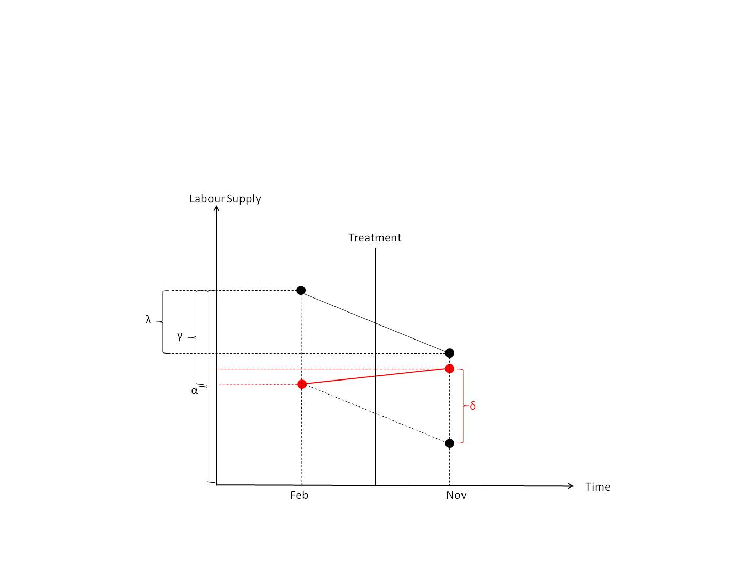
\includegraphics[scale=0.90]{./lecture_includes/waldinger_dd_5.pdf}
	\end{figure}
\end{frame}


\begin{frame}[plain]
	$$Y_{ist} = \alpha + \gamma NJ_s + \lambda d_t + \delta(NJ\times d)_{st} + \varepsilon_{ist}$$
	\begin{figure}
	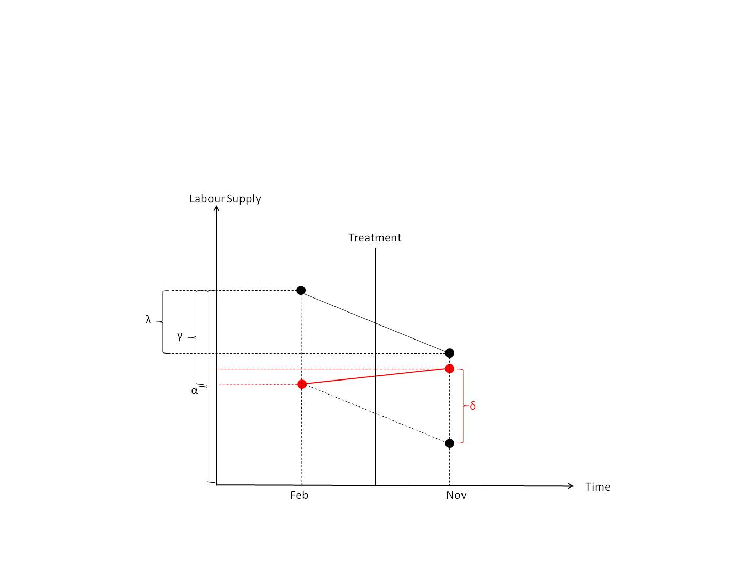
\includegraphics[scale=0.90]{./lecture_includes/waldinger_dd_5.pdf}
	\end{figure}

Notice how OLS is ``imputing'' $\textcolor{red}{\Delta E[Y^0|D=1,Post]}$ for the treatment group across treatment? Parallel trends means $\Delta E[Y^0 |D=0]$ is a valid model of it.

\end{frame}

\subsection{Inference}

\begin{frame}{Inference}
	
	\begin{itemize}
	\item Until recently, most popular work on DiD came from Bertrand, Duflo and Mullainthan (2004) to do with standard errors being too small
	\item They show that conventional standard errors will often severely understate the standard deviation of the estimators
	\item They proposed some solutions -- namely block bootstrapping and clustering (their third one is weird)
	\end{itemize}
\end{frame}


\begin{frame}{Inference}
	
		\begin{enumerate}
		\item[1 ] Block bootstrapping standard errors (if you analyze states the block should be the states and you would sample whole states with replacement for bootstrapping)
		\item[2 ] Clustering standard errors at the group level (in Stata one would simply add \texttt{, cluster(state)} to the regression equation if one analyzes state level variation)
		\end{enumerate}

\bigskip

Most people will simply cluster, but there are issues if you have too few clusters. 
		
\end{frame}




\section{Parallel trends violations}

\subsection{How parallel trends can get violated}


\begin{frame}{Violating parallel trends exercise}

\begin{itemize}
\item Parallel trends means when we impute the missing $\textcolor{red}{\Delta E[Y^0|D=1]}$ with $E[Y^0|D=0]$ either explicitly or implicitly, it ``works''
\item Which means if parallel trends isn't true, then the imputation isn't correct and therefore estimates are biased
\end{itemize}

\end{frame}


\begin{frame}{Violating parallel trends}

\begin{itemize}
\item Parallel trends are in expectation only -- we don't rely everybody to follow the same trend, just that the group average for $Y^0$ be approximately the same for treated and control 
\item Violations are a form of selection bias and there are two straightforward ways that parallel trends will be violated
	\begin{enumerate}
	\item Compositional differences in samples associated with repeated cross-sections
	\item Policy endogeneity
	\end{enumerate}
\end{itemize}

\end{frame}



\begin{frame}{Repeated cross-sections and compositional change}
	
	\begin{itemize}
	\item One of the risks of a repeated cross-section is that the composition of the sample may have changed between the pre and post period in ways that are correlated with treatment
	\item Hong (2013) uses repeated cross-sectional data from the Consumer Expenditure Survey (CEX) containing music expenditure and internet use for a random sample of households
	\item Study exploits the emergence of Napster (first file sharing software widely used by Internet users) in June 1999 as a natural experiment
	\item Study compares internet users and internet non-users before and after emergence of Napster
	\end{itemize}

\end{frame}

\begin{frame}[plain]
	\begin{figure}
	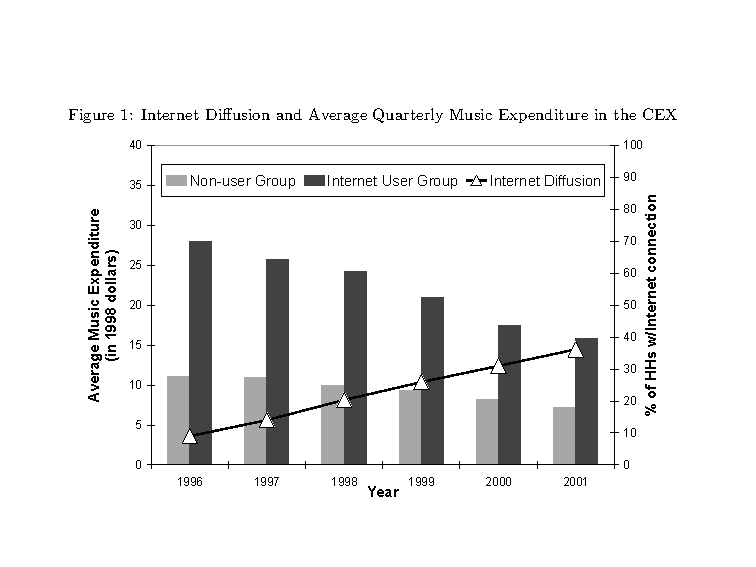
\includegraphics{./lecture_includes/Hong_1.pdf}
	\end{figure}
	
\end{frame}

\begin{frame}[shrink=20,plain]
	\begin{figure}
	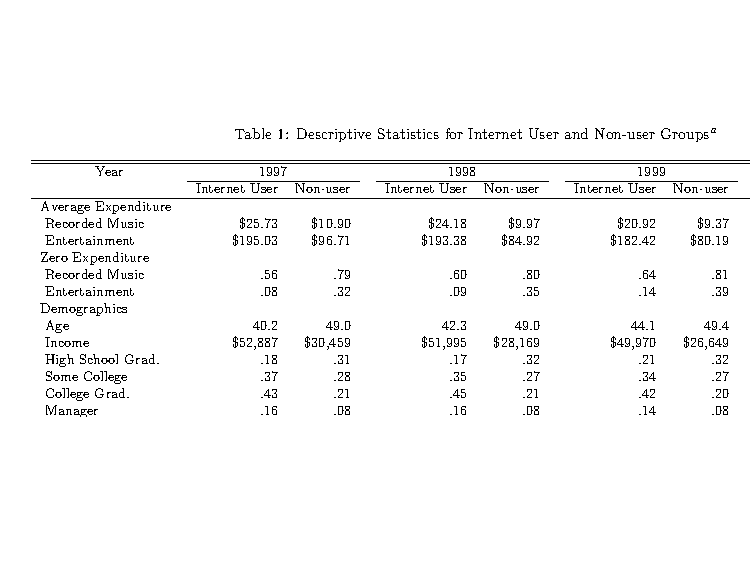
\includegraphics{./lecture_includes/Hong_2.pdf}
	\end{figure}
	
	Diffusion of the Internet changes samples (e.g., younger music fans are early adopters)
	
\end{frame}

\begin{frame}{Repeated cross-sections}

\begin{itemize}
\item Surprisingly under-appreciated problem with almost no literature around it
\item So what can you do?  Check covariate balance by regressing the time-varying covariates instead of the outcome onto the treatment using your OLS specification
\item They should be exogenous remember, so this covariate regression can be a helpful test of whether this is a problem
\item Hong proposed a propensity score model to create balance on covariates to address this underlying sample selection problem
\end{itemize}

\end{frame}


\subsection{Example of a great DiD}

\begin{frame}{Types of evidence}

\begin{itemize}
\item You are building a case, the prosecutor before a judge and jury, always in battle with the defense attorney
\item Evidence has particular broadly defined forms that can help you on the front end
\item Your goal in my humble opinion should be mixing tight logic based falsifications with particular kinds of data visualization, starting with the event study
\end{itemize}

\end{frame}


\begin{frame}{Event studies have become mandatory in DiD}

	\begin{figure}
	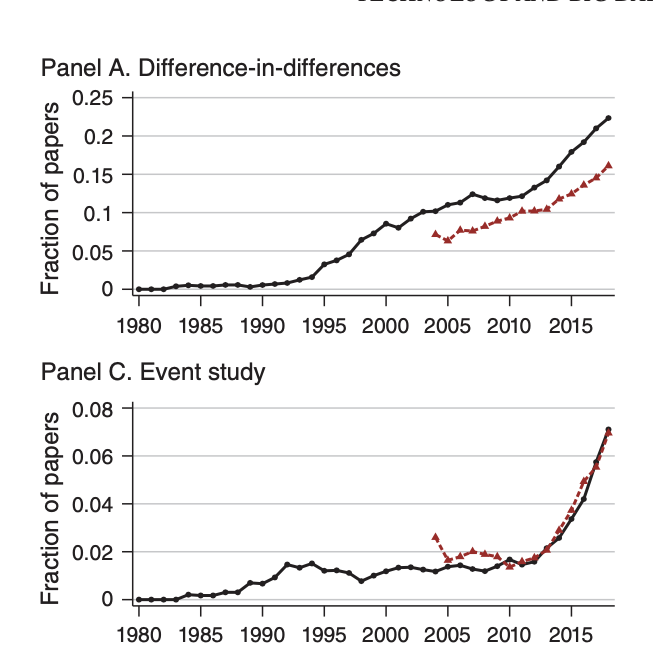
\includegraphics[scale=0.5]{./lecture_includes/currie_eventstudy.png}
	\end{figure}

\end{frame}

\begin{frame}{Intuition behind event studies}

\begin{itemize}
	\item Princeton Industrial Relations Section seems to be behind this -- this intense focus on research design but also verifying assumptions
	\item The identifying assumption for all DD designs is parallel trends , but since we cannot verify parallel trends, we often look at pre-trends
	\item It's a type of check for selection bias, but you must understand what it is and what it isn't to see its value but not be naive about it (it is not a silver bullet)
	\item Even if pre-trends are the same one still has to worry about other policies changing at the same time (omitted variable bias is a parallel trends violation)

\end{itemize}

\end{frame}




\begin{frame}{Plot the raw data when there's only two groups}

	\begin{figure}
	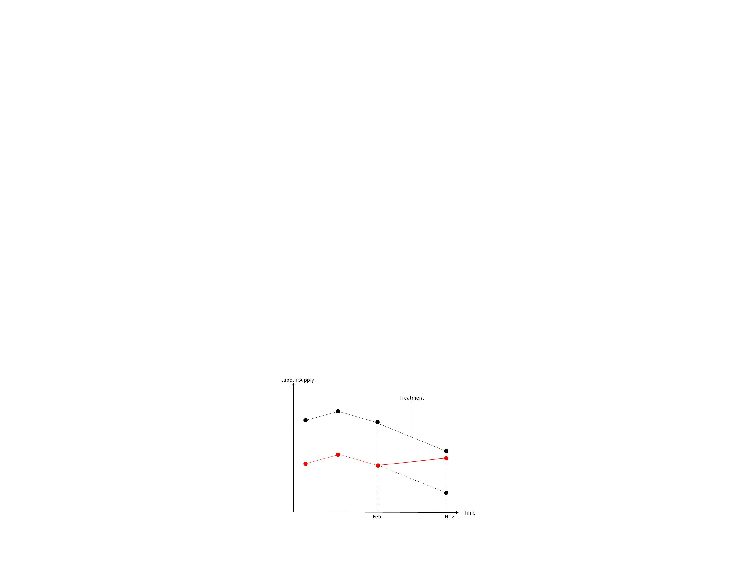
\includegraphics[scale=2.5]{./lecture_includes/waldinger_dd_6.pdf}
	\end{figure}

\end{frame}


\begin{frame}{Beware of naive reasoning}

\begin{itemize}
\item Parallel pre-trends $\neq$ parallel trends -- these are often thought to be the same thing, and they aren't
\item Equating them is a kind of \emph{post hoc ergo propter hoc} fallacy
\item Parallel pre-trends is more like a smoking gun based on things ``looking the same'' before
\item Similar to checking for covariate balance in RCTs
\item But \textbf{cannot} substitute for domain knowledge!
\end{itemize}

\end{frame}


\begin{frame}{Event study regression}
	
	\begin{itemize}
	\item Event studies have a simple OLS specification with only one treatment group and one never-treated group $$Y_{its} = \alpha +  \sum_{\tau=-2}^{-q}\mu_{\tau}D_{s\tau} + \sum_{\tau=0}^m\delta_{\tau}D_{s\tau}+\varepsilon_{ist}$$
		\begin{itemize}
		\item where $D$ is an interaction of the treatment group $s$ with the calendar year $\tau$
		\item Treatment occurs in year 0, no anticipation, drop baseline $t-1$
		\item Includes $q$ leads or anticipatory effects and $m$ lags or post treatment effects
		\end{itemize}
	\end{itemize}
\end{frame}

\begin{frame}{Event study regression}


$$Y_{its} = \alpha + \sum_{\tau=-2}^{-q}\mu_{\tau}D_{s\tau} + \sum_{\tau=0}^m\delta_{\tau}D_{s\tau}+\varepsilon_{ist}$$

\bigskip

Typically you'll plot the coefficients and 95\% CI on all leads and lags (binned or not, trimmed or not) 

\bigskip

Under no anticipation, then you expect $\widehat{\mu}$ coefficients to be zero, which gives you confidence that parallel trends holds (but is not a guarantee, and there are still specification issues -- see Jon Roth's work)

\bigskip

Under parallel trends, $\widehat{\delta}$ are estimates of the ATT at points in time

\end{frame}



\begin{frame}{Medicaid and Affordable Care Act example}

\begin{figure}

\includegraphics[scale=0.25]{./lecture_includes/medicaid_qje}
\end{figure}

\end{frame}

\begin{frame}{Types of evidence}

\begin{itemize}
\item \textbf{Bite} -- show that the expansion shifted people into Medicaid and out of uninsured status
\item \textbf{Placebos} -- Show that there's no effect on mortality for groups it shouldn't be affecting (people 65+)
\item \textbf{Event study} -- Show leads and lags on mortality
\end{itemize}

\end{frame}


\imageframe{./lecture_includes/Miller_Medicaid1.png}

\imageframe{./lecture_includes/Miller_Medicaid2.png}

\imageframe{./lecture_includes/Miller_Medicaid3.png}

\begin{frame}[plain]

	\begin{figure}

	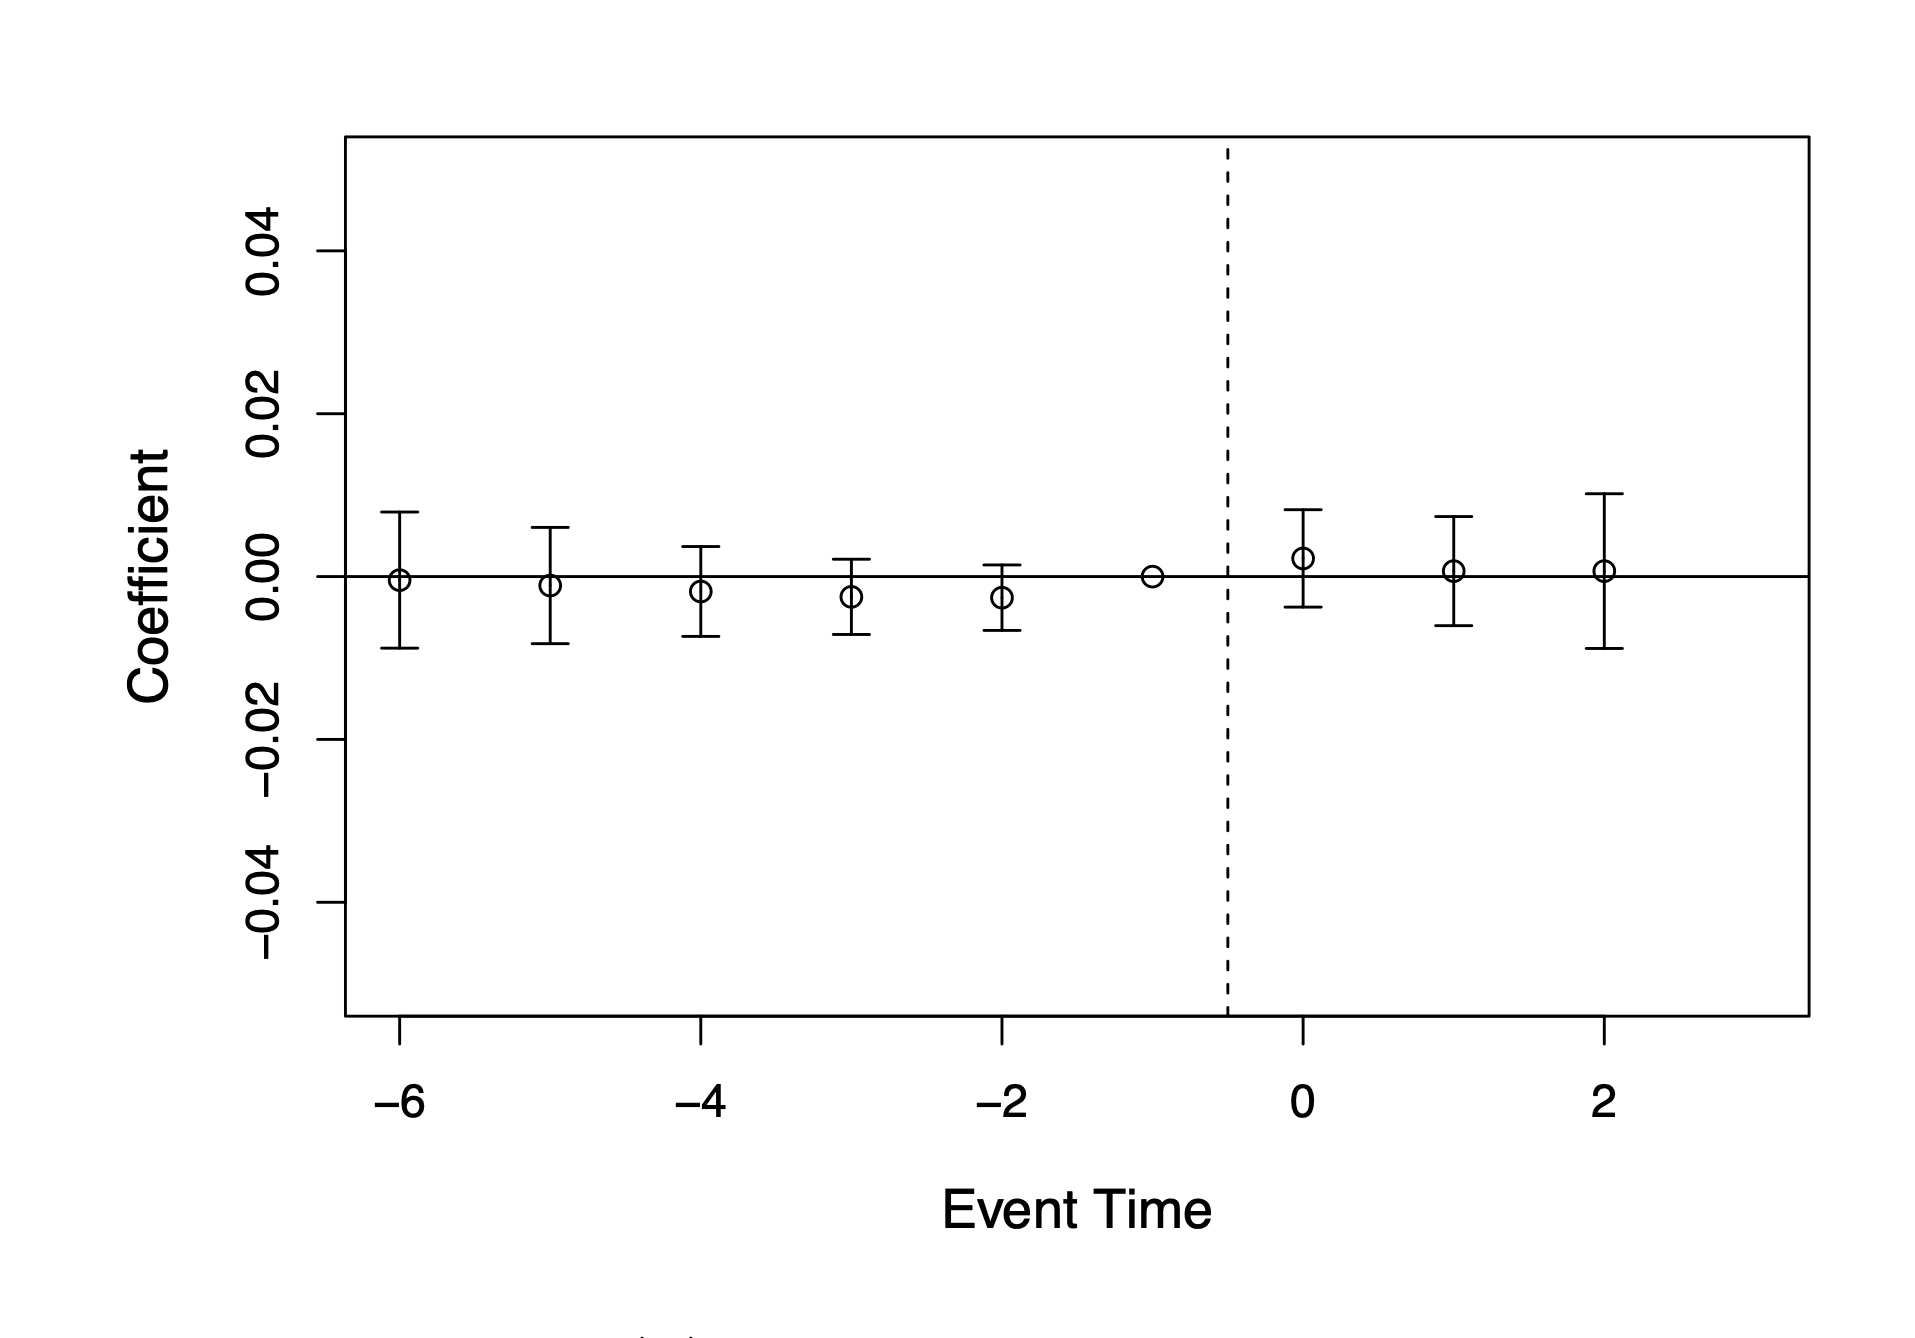
\includegraphics[scale=0.3]{./lecture_includes/medicaid_qje_placebo}
	\caption{Miller, et al. (2019) estimates of Medicaid expansion's effects on on 65 yo and older mortality}
	\end{figure}

\end{frame}

\begin{frame}[plain]

	\begin{figure}
	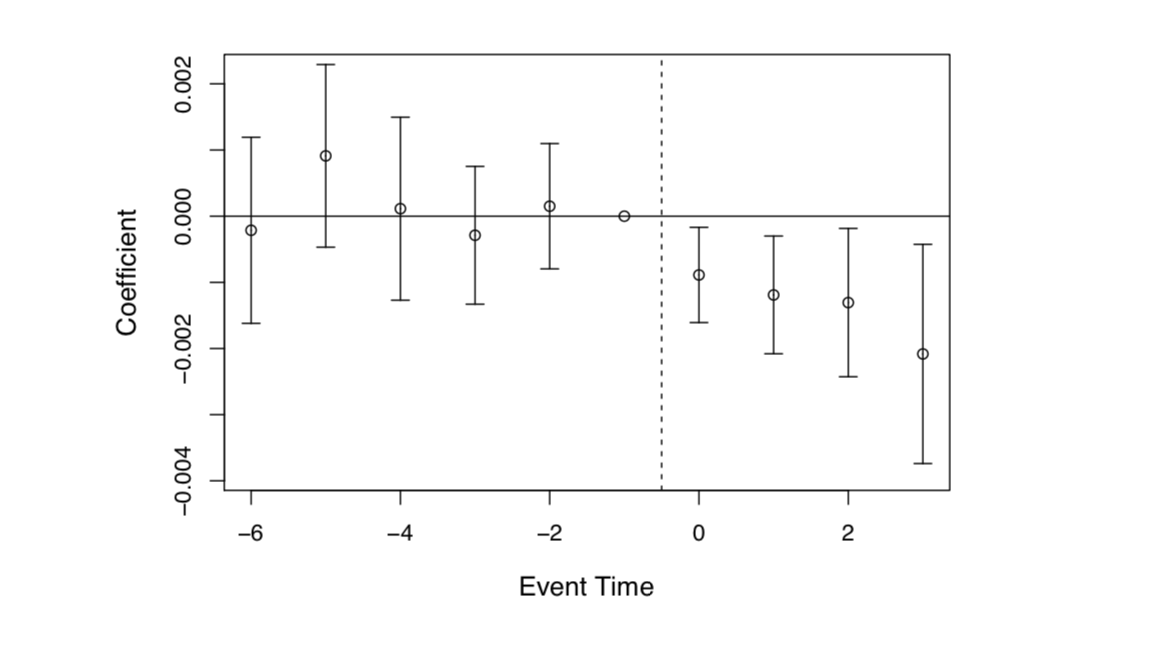
\includegraphics[scale=0.3]{./lecture_includes/Miller_Medicaid4.png}
	\caption{Miller, et al. (2019) estimates of Medicaid expansion's effects on on annual mortality}
	\end{figure}

\end{frame}



\section{Differential timing}

\subsection{Bacon decomposition}

\begin{frame}{Differential timing}

\begin{itemize}
\item So far we have been covering the simpler case with two groups (one treated, one not treated)
\item In the two group case, we only need parallel trends to identify the ATT and can use OLS with unit and time fixed effects since it'll calculate the means needed for DiD equation
\item Now let's move to a very common scenario in which more than two groups are treated at different times
\end{itemize}

\end{frame}

\begin{frame}{Modeling outcomes with TWFE versus DiD}

\begin{equation}
Y_{it} = \alpha_0 + \delta D_{it} + \sigma_i + \tau_t + \varepsilon_{it}
\end{equation}

\bigskip


This is slightly different than OLS; no interaction. And $\delta$ is assumed to be constant.  Developed to model outcome as function of time invariant unobserved heterogeneity, but was applied to DiD once researchers began using more complex designs (differential timing). Now called twoway fixed effects (TWFE)

\bigskip

TWFE models outcomes as a function of time invariant heterogeneity (eliminated with fixed effects). Listen to Angrist.

\url{https://www.youtube.com/watch?v=J1o45BXY5X4}


\end{frame}

\begin{frame}{2x2 versus differential timing}

\begin{itemize}
	\item We will first decompose TWFE using the Bacon decomposition to understand what it needs for unbiasedness under differential timing (but there are other decompositions)
	\item This exposition is from Goodman-Bacon (2022) but the expression of the weights is from 2018 for personal preference
	\item Goodman-Bacon (2022) is influential because of the clarity showing that parallel trends is \textbf{not enough} for TWFE to be unbiased when treatment adoption is described by differential timing
\end{itemize}

\end{frame}


\begin{frame}{TWFE}


\begin{itemize}
\item Very old model, going back to the mid-1900s (Eisenhart 1947, Scheffe 1956)
\item Panel econometrics which models constant heterogeneity as a nuisance term that can be eliminated through demeaning
\item Not sure when it gets brought into diff-in-diff but in the mid-1990s panel fixed effects was the dominant model (see Lott and Mustard 1997) and the words ``difference-in-differences'' weren't always used
\end{itemize}

\end{frame}

\begin{frame}{Fixed effects}
	
Running a regression with the time-demeaned variables $\ddot{y}_{it}\equiv y_{it} - \bar{y}_i$ and $\ddot{x}_{it} \equiv x_{it} - \bar{x}$ is numerically equivalent to a regression of $y_{it}$ on $x_{it}$ and unit specific dummy variables.

\bigskip

Even better, the regression with the time demeaned variables is consistent for $\beta$ even when $Cov[x_{it},c_i]\neq 0$ because time-demeaning eliminates the unobserved effects

\begin{eqnarray*}
y_{it} &=& x_{it}\beta + c_i + \varepsilon_{it} \\
\bar{y}_i &=& \bar{x}_i \beta + c_i + \bar{\varepsilon}_{i}\\
\hline \\
(y_{it} - \bar{y}_i) &=& (x_{it} - \bar{x})\beta + (c_i - c_i) + (\varepsilon_{it} - \bar{\varepsilon}_i) \\
\ddot{y}_{it} &=& \ddot{x}_{it}\beta + \ddot{\varepsilon}_{it}
\end{eqnarray*}

\end{frame}

\begin{frame}{Fixed effects}
	
	\begin{itemize}
	\item Identification assumptions:	
		\begin{enumerate}
		\item $E[\varepsilon_{it} | x_{i1}, x_{i2}, \dots, x_{iT}, c_i]=0; t=1,2,\dots,T$
			\begin{itemize}
			\item regressors are strictly exogenous conditional on the unobserved effect
			\item allows $x_{it}$ to be arbitrarily related to $c_i$
			\end{itemize}
		\item $rank\bigg( \sum_{t=1}^T E[\ddot{x}_{it}'\ddot{x}_{it}]\bigg) = K$
			\begin{itemize}
			\item regressors vary over time for at least some $i$ and not collinear
			\end{itemize}
		\end{enumerate}
	\item Fixed effects estimator
		\begin{enumerate}
		\item Demean and regress $\ddot{y}_{it}$ on $\ddot{x}_{it}$ (need to correct degrees of freedom)
		\item Regress $y_{it}$ on $x_{it}$ and unit dummies (dummy variable regression)
		\item Regress $y_{it}$ on $x_{it}$ with canned fixed effects routine
			\begin{itemize}
			\item Stata: \texttt{xtreg y x, fe i(PanelID)}
			\end{itemize}
		\end{enumerate}
	\end{itemize}
\end{frame}


\begin{frame}{Fixed effects}

\begin{itemize}
	\item Properties (under assumptions 1-2):
		\begin{itemize}
		\item $\widehat{\beta}_{FE}$ is consistent: $\underset{N\rightarrow \infty}{plim} \widehat{\beta}_{FE,N}=\beta$
		\item $\widehat{\beta}_{FE}$ is unbiased conditional on \textbf{X}
		\end{itemize}
\item TWFE model identifies causal effect if strict exogeneity holds
\item What is strict exogeneity in words? Policy endogeneity? Parallel trends? No potential outcomes; only realized outcomes
\end{itemize}

\end{frame}


\begin{frame}{Strict exogeneity violation}

\begin{itemize}
\item As it turns out, with differential timing, strict exogeneity was violated if there was heterogeneity as the heterogeneity was correlated with fixed effects and became absorbed in the error term (Gardner 2021)
\item But this was not well understood if at all until Borusyak and Jaravel (2016) and others
\item There's a few decompositions out there but Bacon's decomposition is first and foremost numerical which allows us to trace back to the spreadsheet calculations.
\end{itemize}

\end{frame}


\begin{frame}{Two decompositions}

\begin{enumerate}
\item \textbf{Bacon numerical decomposition}: Show that the estimated regression coefficient once time and panel fixed effects are partialed out can be interpreted as a weighted average over all possible diff-in-diff equations (or 2x2s)
\item \textbf{Bacon potential outcome decomposition}: Using switching equation to replace realized outcomes with potential outcomes, we can see that TWFE is biased both by parallel trends and dynamic treatment effects
\end{enumerate}

\end{frame}



\begin{frame}{Bacon Numerical Decomposition Preview}

\begin{itemize}
\item TWFE estimates a parameter that is a weighted average over all 2x2 in your sample
\item TWFE assigns weights that are a function of sample sizes of each ``group'' and the variance of the treatment dummies for those groups
\end{itemize}

\end{frame}

\begin{frame}{Bacon Potential Outcome Decomposition Preview}

\begin{itemize}
\item TWFE needs two assumptions: that the variance weighted parallel trends are zero (far more parallel trends iow) and no dynamic treatment effects (not the case with 2x2)
\item Under those assumptions, TWFE estimator estimates the variance weighted ATT as a weighted average of all possible ATTs
\end{itemize}

\end{frame}


\begin{frame}{$K^2$ distinct DDs}

Let's look at 3 timing groups (a, b and c) and one untreated group (U).  With 3 timing groups, there are 9 2x2 DDs.  Here they are:


\begin{center}
\begin{tabular}{c|c|c}
\multicolumn{1}{l}{} &
\multicolumn{1}{l}{} &
\multicolumn{1}{l}{} \\
\midrule
a to b & b to a & c to a \\
a to c & b to c & c to b \\
a to U & b to U & c to U \\
\midrule
\end{tabular}
\end{center}

\bigskip

Let's return to a simpler example with only two groups -- a $k$ group treated at $t_k^*$ and an $l$ treated at $t_l^*$ plus an never-treated group called the $U$ untreated group
\end{frame} 


\begin{frame}{Terms and notation}

\begin{itemize}
\item Let there be two treatment groups (k,l) and one untreated group (U)
\item k,l define the groups based on when they receive treatment (differently in time) with k receiving it earlier than l
\item Denote $\overline{D}_k$ as the share of time each group spends in treatment status
\item Denote $\widehat{\delta}_{jb}^{2x2}$ as the canonical $2\times 2$ DD estimator for groups $j$ and b where $j$ is the treatment group and $b$ is the comparison group
\end{itemize}

\end{frame}


\imageframe{./lecture_includes/bacon_goodman_2.png}



\begin{frame}[plain]
$$\widehat{\delta}^{2x2}_{kU} = \bigg ( \overline{y}_k^{post(k)} - \overline{y}_k^{pre(k)} \bigg ) - \bigg ( \overline{y}_U^{post(k)} - \overline{y}_U^{pre(k)} \bigg ) $$
	\begin{figure}
	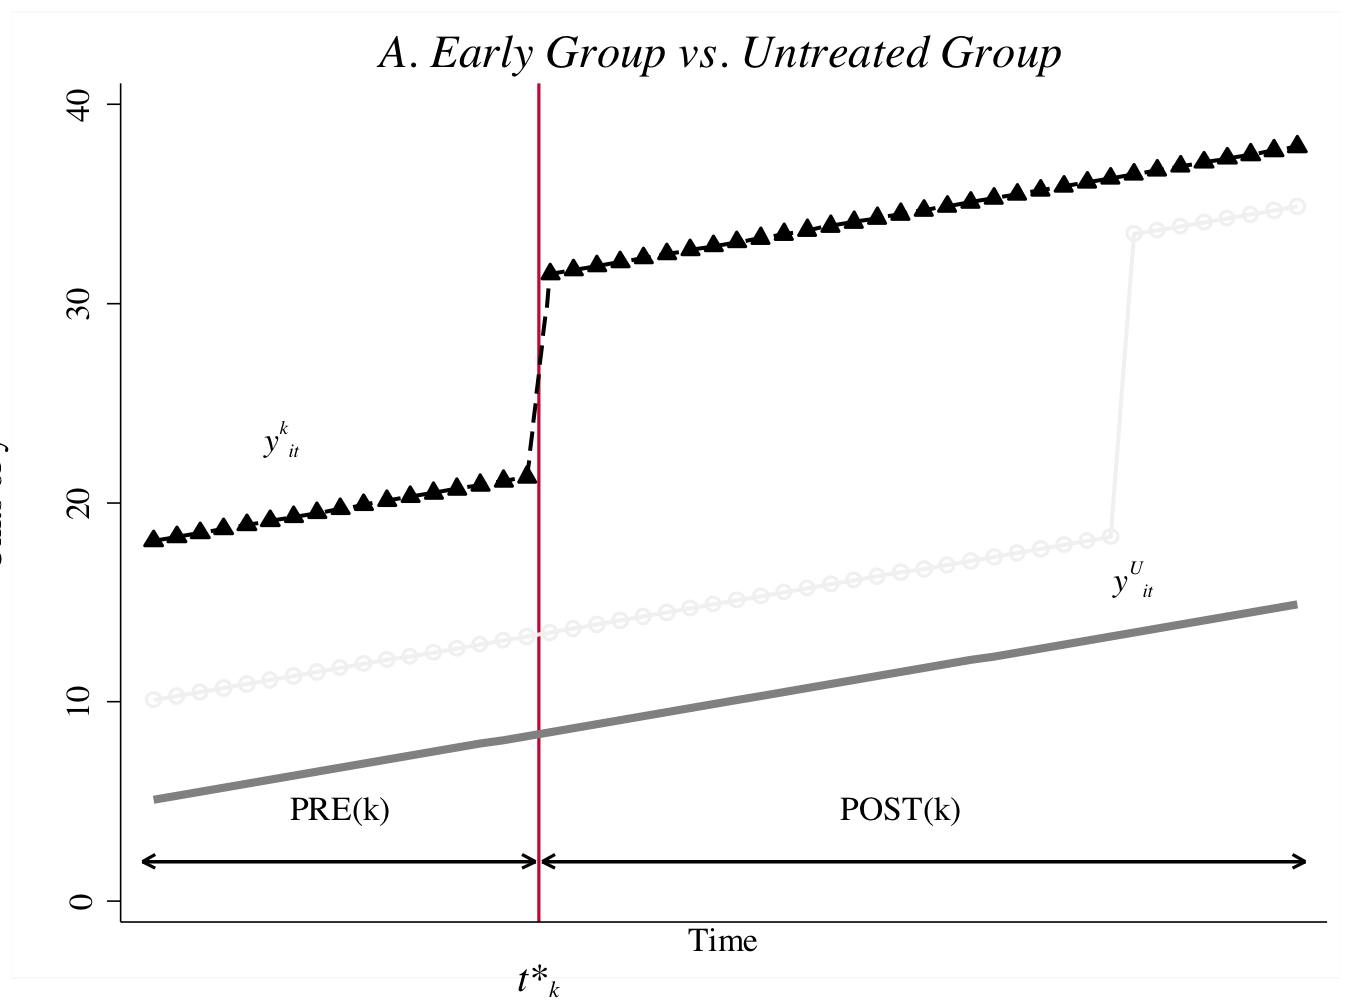
\includegraphics[scale=0.45]{./lecture_includes/bacon_goodman_3.png}
	\end{figure}

\end{frame}

\begin{frame}[plain]
$$\widehat{\delta}^{2x2}_{lU} = \bigg ( \overline{y}_l^{post(l)} - \overline{y}_l^{pre(l)} \bigg ) - \bigg ( \overline{y}_U^{post(l)} - \overline{y}_U^{pre(l)} \bigg ) $$
	\begin{figure}
	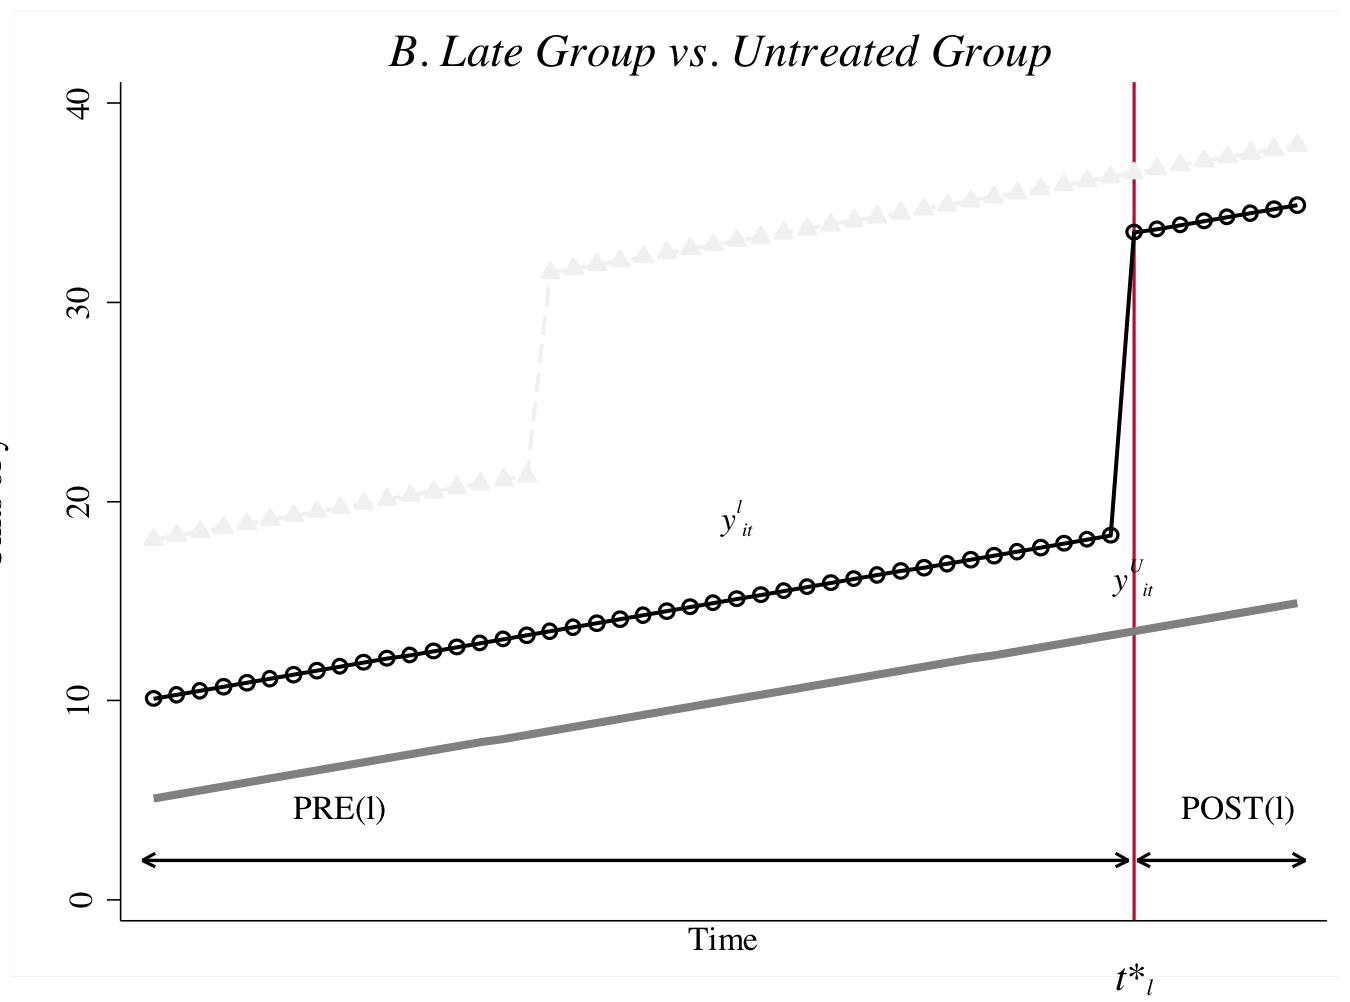
\includegraphics[scale=0.45]{./lecture_includes/bacon_goodman_4.png}
	\end{figure}

\end{frame}


\begin{frame}[plain]

$$\delta_{kl}^{2x2,k} = \bigg ( \overline{y}_k^{MID(k,l)} - \overline{y}_k^{Pre(k,l)} \bigg ) - \bigg ( \overline{y}_l^{MID(k,l)} - \overline{y}_l^{PRE(k,l)} \bigg ) $$

	\begin{figure}
	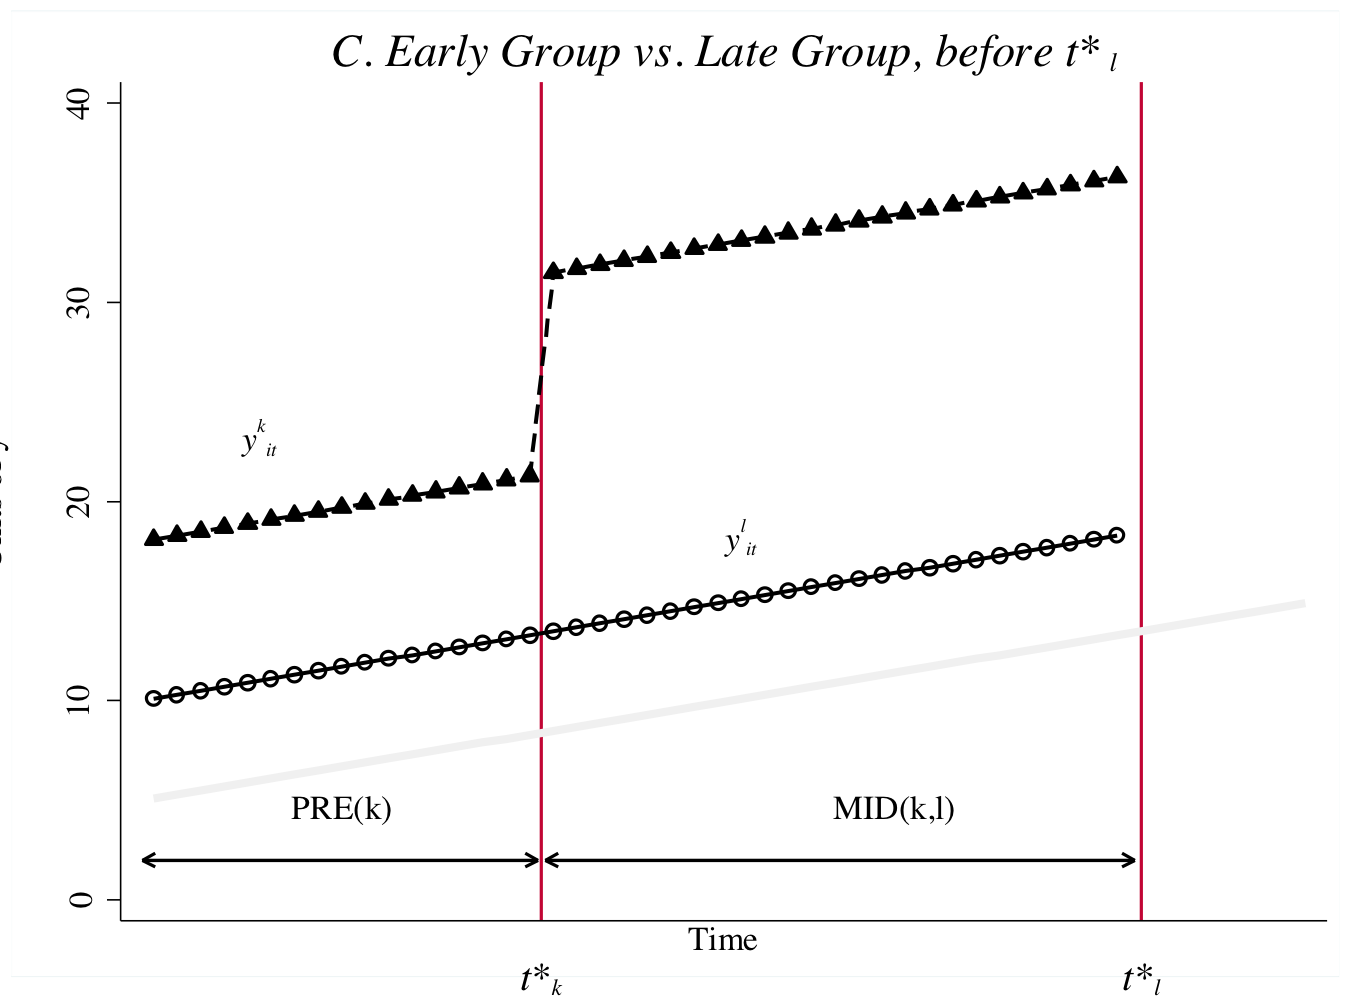
\includegraphics[scale=0.45]{./lecture_includes/bacon_goodman_6.png}
	\end{figure}

\end{frame}

\begin{frame}[plain]
$$\delta_{lk}^{2x2,l} = \bigg ( \overline{y}_l^{POST(k,l)} - \overline{y}_l^{MID(k,l)} \bigg ) - \bigg ( \overline{y}_k^{POST(k,l)} - \overline{y}_k^{MID(k,l)} \bigg ) $$

	\begin{figure}
	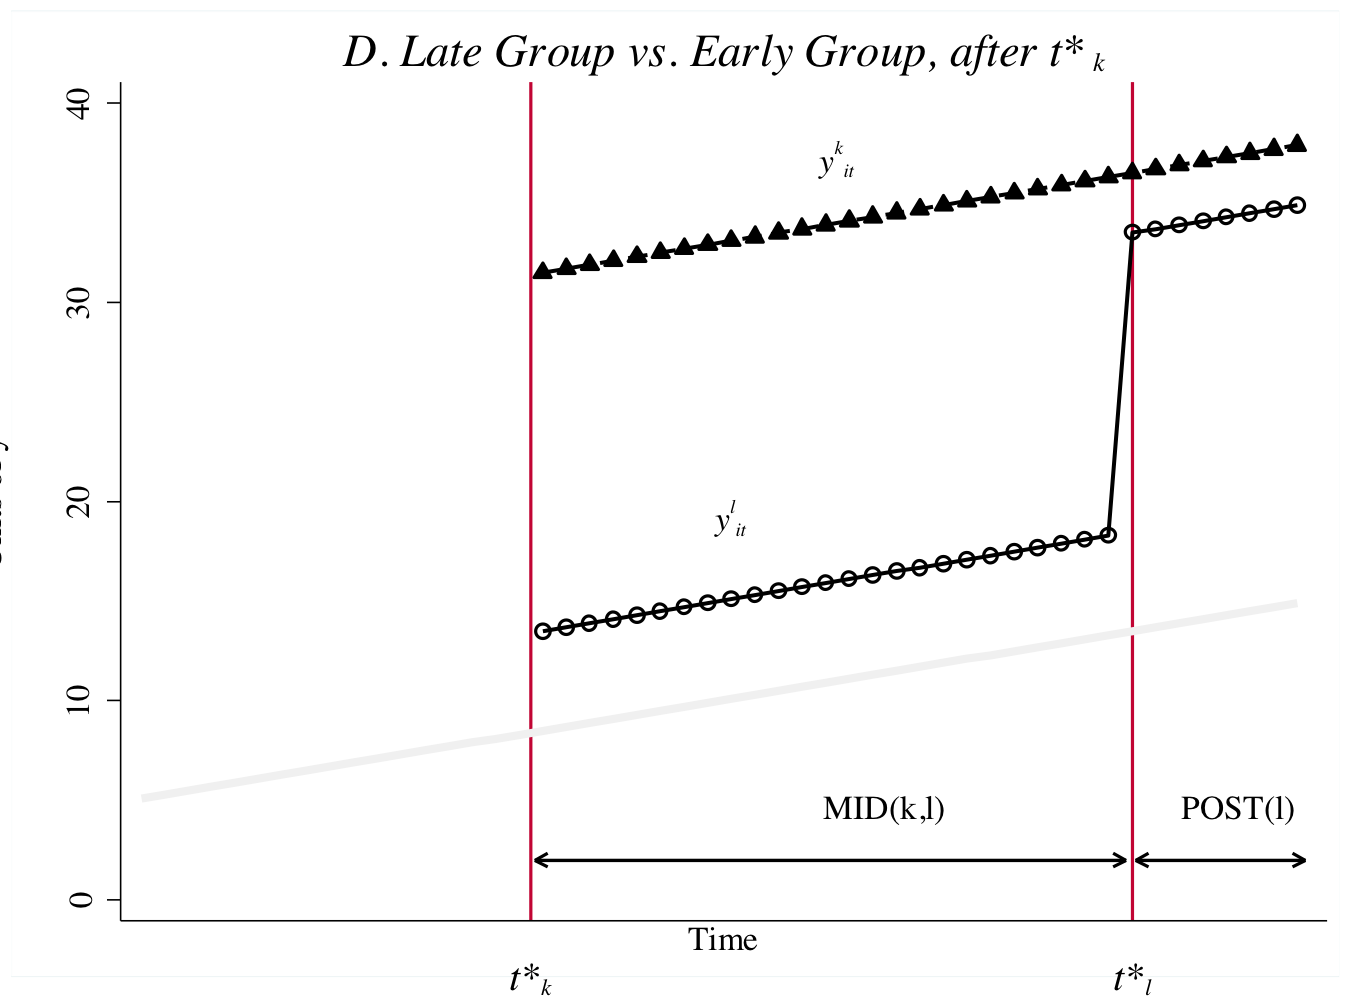
\includegraphics[scale=0.4]{./lecture_includes/bacon_goodman_7.png}
	\end{figure}

\end{frame}


%\begin{frame}[plain]
%\begin{center}
%\textbf{Typical regression equation}
%\end{center}

%$$y_{it}  =  \delta D_{it}  + \alpha_i + \alpha_t + \epsilon_{it}$$

%\begin{enumerate}
%\item Partial out the fixed effects (Frisch-Waugh-Lovell theorem) 
%	\begin{eqnarray*}
%	\tilde{D}_{it} = (D_{it} - \overline{\overline{D}} ) - (\overline{D}_i - \overline{\overline{D}}) - (\overline{D}_t - \overline{\overline{D}} )\\
%	\tilde{y}_{it} = (D_{it} - \overline{\overline{y}} ) - (\overline{y}_i - \overline{\overline{y}}) - (\overline{y}_t - \overline{\overline{y}})
%	\end{eqnarray*}where $\overline{\overline{x}} = \frac{1}{NT}\sum_i \sum_t x_{it}$
%\item Calculate univariate coefficient by brute force
%$$\widehat{\delta}^{DD} = \frac{ \widehat{Cov}(\tilde{D}_{it}, \tilde{y}_{it})}{\widehat{Var}(\tilde{D}_{it})} = \frac{ \frac{1}{NT} \sum_i \sum_t (y_{it} - \overline{\overline{y}})(D_{it} - \overline{\overline{D}})}{ \frac{1}{NT} \sum_i \sum_t (D_{it} - \overline{\overline{D}} ) }$$
%\end{enumerate}

%\end{frame}
	

\begin{frame}{Bacon decomposition}


TWFE estimate yields a weighted combination of each groups' respective 2x2 (of which there are 4 in this example)
\begin{eqnarray*}	
\widehat{\delta}^{DD} = \sum_{k \neq U} s_{kU}\widehat{\delta}_{kU}^{2x2} + \sum_{k \neq U} \sum_{l>k} s_{kl}  \bigg [ \mu_{kl}\widehat{\delta}_{kl}^{2x2,k} + (1-\mu_{kl}) \widehat{\delta}_{lk}^{2x2,l} \bigg]
\end{eqnarray*}where that first 2x2 combines the k compared to U and the l to U (combined to make the equation shorter)

\end{frame}
	


\begin{frame}{Third, the Weights}

 \begin{eqnarray*} s_{ku} &=& \frac{ n_k n_u \overline{D}_k (1- \overline{D}_k ) }{ \widehat{Var} ( \tilde{D}_{it} )} \\
s_{kl} &=& \frac{ n_k n_l (\overline{D}_k - \overline{D}_{l} ) ( 1- ( \overline{D}_k - \overline{D}_{l} )) }{\widehat{Var}(\tilde{D}_{it})} \\
\mu_{kl} &=& \frac{1 - \overline{D}_k }{1 - ( \overline{D}_k - \overline{D}_{l} )}
\end{eqnarray*}where $n$ refer to sample sizes, $\overline{D}_k (1- \overline{D}_k )$ $(\overline{D}_k - \overline{D}_{l} ) ( 1- ( \overline{D}_k - \overline{D}_{l} ))$ expressions refer to variance of treatment, and the final equation is the same for two timing groups.

\end{frame}

\begin{frame}{Weights discussion}

\begin{itemize}
\item Two things to note:
	\begin{itemize}
	\item More units in a group, the bigger its 2x2 weight is
	\item Group treatment variance weights up or down a group's 2x2
	\end{itemize}
\item Bacon notes that since variation comes from the group not the unit, better to include group-trends not unit trends 
\item Group treatment variance as a weight is probably the most surprising part of the weighting scheme
\end{itemize}
\end{frame}


\begin{frame}{Weights discussion}

\begin{itemize}
\item Notice the quadratic form of the treatment variance $$\overline{D}_k(1-\overline{D}_k)=\overline{D_k}-\overline{D}_k^2$$
\item Choose $\overline{D}_k$ that maximizes that quadratic by taking derivative and setting to zero. 
\item Let's illustrate it numerically
	\begin{itemize}
	\item $\overline{D}=0.1$. Then $0.1 \times 0.9 = 0.09$
	\item $\overline{D}=0.4$. Then $0.4 \times 0.6 =0.24$
	\item $\overline{D}=0.5$. Then $0.5 \times 0.5 = 0.25$
	\item $\overline{D}=0.6$. Then $0.6 \times 0.4 = 0.24$
	\end{itemize}
\item This means the weight on treatment variance is maximized for \emph{groups treated in middle of the panel}
\end{itemize}
\end{frame}

\begin{frame}{More weights discussion}

\begin{itemize}
\item But what about the ``treated on treated'' weights (i.e., $\overline{D}_k - \overline{D}_{l} $)  
\item Same principle as before - when the difference between treatment variance is close to 0.5, those 2x2s are given the greatest weight
\item For instance, say $t^*_k=0.15$ and $t^*_l=0.67$. Then $\overline{D}_k - \overline{D}_{l} = 0.52$.  And thus $0.52 \times 0.48 = 0.2496$.
\end{itemize}

\end{frame}


\begin{frame}{Summarizing TWFE centralities}

\begin{itemize}
\item Groups in the middle of the panel weight up their respective 2x2s via the variance weighting
\item Decomposition highlights the strange role of panel length when using TWFE
\item Different choices about panel length change both the 2x2 and the weights based on variance of treatment
\end{itemize}

\end{frame}

%\begin{frame}[plain]
%\begin{center}
%\textbf{DD Decomposition Theorem}
%\end{center}

%Assume that there are $k=1,\dots,K$ groups of treated units ordered by treatment time $_k^*$ and one control group $U$ which does not receive treatment in the data.  The share of units in group $k$ is $n_k$ and the share of periods that group $k$ spends under treatment is $\overline{D}_k$. The DD estimate from a two-way fixed effects model is a weighted average of all two-group DD estimators.

%\begin{eqnarray*}
%\widehat{\delta}^{DD} = \sum_{k \neq u} s_{ku} \widehat{\delta}_{ku}^{DD} + \sum_{k \neq u} \sum_{l > k} s_{kl} \bigg [ \mu_{kl} \widehat{\delta}_{kl}^{DD,k} + (1-\mu_{kl} ) \widehat{\delta}_{kl}^{DD,l} \bigg ]
%\end{eqnarray*}with weights equal to  \begin{eqnarray*} s_{ku} &=& \frac{ n_k n_u \overline{D}_k (1- \overline{D}_k ) }{ \widehat{Var} ( \tilde{D}_{it} )} \\
%s_{kl'} &=& \frac{ n_k n_l (\overline{D}_k - \overline{D}_{l} ) ( 1- ( \overline{D}_k - \overline{D}_{l} )) }{\widehat{Var}(\tilde{D}_{it})} \\
%\mu_{kl} &=& \frac{1 - \overline{D}_k }{1 - ( \overline{D}_k - \overline{D}_{j'} )}
%\end{eqnarray*}

%\end{frame}

\begin{frame}{Moving from 2x2s to causal effects and bias terms}

Let's start breaking down these estimators into their corresponding estimation objects expressed in causal effects and biases


\begin{eqnarray*}
\widehat{\delta}^{2x2}_{kU} &=& ATT_k{Post} + \Delta Y^0_k(Post(k),Pre(k)) - \Delta Y^0_U(Post(k),Pre) \\
\widehat{\delta}^{2x2}_{kl} &=& ATT_k(MID) + \Delta Y^0_k(MID,Pre) - \Delta Y^0_l(MID, Pre)
\end{eqnarray*}These look the same because you're always comparing the treated unit with an untreated unit (though in the second case it's just that they haven't been treated \emph{yet}). 

\end{frame}

\begin{frame}{The dangerous 2x2}

But what about the 2x2 that compared the late groups to the already-treated earlier groups? With a lot of substitutions we get:

\begin{eqnarray*}
\widehat{\delta}^{2x2}_{lk} &=& ATT_{l,Post(l)} + \underbrace{\Delta Y^0_l(Post(l),MID) - \Delta Y^0_k ( Post(l), MID)}_{\mathclap{\text{Parallel trends bias}}} \\
&& - \underbrace{(ATT_k(Post) - ATT_k(Mid))}_{\mathclap{\text{Heterogeneity bias!}}}
\end{eqnarray*}


\end{frame}

\begin{frame}{Substitute all this stuff into the decomposition formula}

\begin{eqnarray*}	
\widehat{\delta}^{DD} = \sum_{k \neq U} s_{kU}\widehat{\delta}_{kU}^{2x2} + \sum_{k \neq U} \sum_{l>k} s_{kl}  \bigg [ \mu_{kl}\widehat{\delta}_{kl}^{2x2,k} + (1-\mu_{kl}) \widehat{\delta}_{kl}^{2x2,l} \bigg]
\end{eqnarray*}where we will make these substitutions\begin{eqnarray*}
\widehat{\delta}_{kU}^{2x2} &=& ATT_k(Post) + \Delta Y_l^0(Post,Pre) - \Delta Y_U^0(Post, Pre) \\
\widehat{\delta}_{kl}^{2x2,k} &=& ATT_k(Mid) + \Delta Y_l^0(Mid,Pre) - \Delta Y_l^0(Mid, Pre) \\
\widehat{\delta}^{2x2,l}_{lk} &=& ATT_{l}Post(l) + \Delta Y^0_l(Post(l),MID) - \Delta Y^0_k ( Post(l), MID) \\
&&- (ATT_k(Post) - ATT_k(Mid))
\end{eqnarray*}Notice all those potential sources of biases! 

\end{frame}


\begin{frame}{Potential Outcome Notation}

\begin{eqnarray*}
p\text{ }lim\text{ } \widehat{\delta}^{TWFE}_{n\to\infty} &=& VWATT + VWPT - \Delta ATT
\end{eqnarray*}

\begin{itemize}
\item Notice the number of assumptions needed \emph{even} to estimate this very strange weighted ATT (which is a function of how you drew the panel in the first place). 
\item With dynamics, it attenuates the estimate (bias) and can even reverse sign depending on the magnitudes of what is otherwise effects in the sign in a reinforcing direction! 
\item Model can flip signs (does not satisfy a ``no sign flip property'')
\end{itemize}

\end{frame}



\subsection{Simulation}

\begin{frame}{Simulated data}

\begin{itemize}
\item 1000 firms, 40 states, 25 firms per states, 1980 to 2009 or 30 years, 30,000 observations, four groups
\item $E[Y^0]$ satisfies ``strong parallel trends''  (stronger than necessary)

$$Y^0_{ist} = \alpha_i + \gamma_t + \varepsilon_{ist}$$

\item Also no anticipation of treatment effects until treatment occurs but does \emph{not} guarantee homogenous treatment effects
\end{itemize}
\end{frame}



\begin{frame}{Group-time ATT}
       \begin{columns}
          \column{0.38\linewidth}
             \centering
             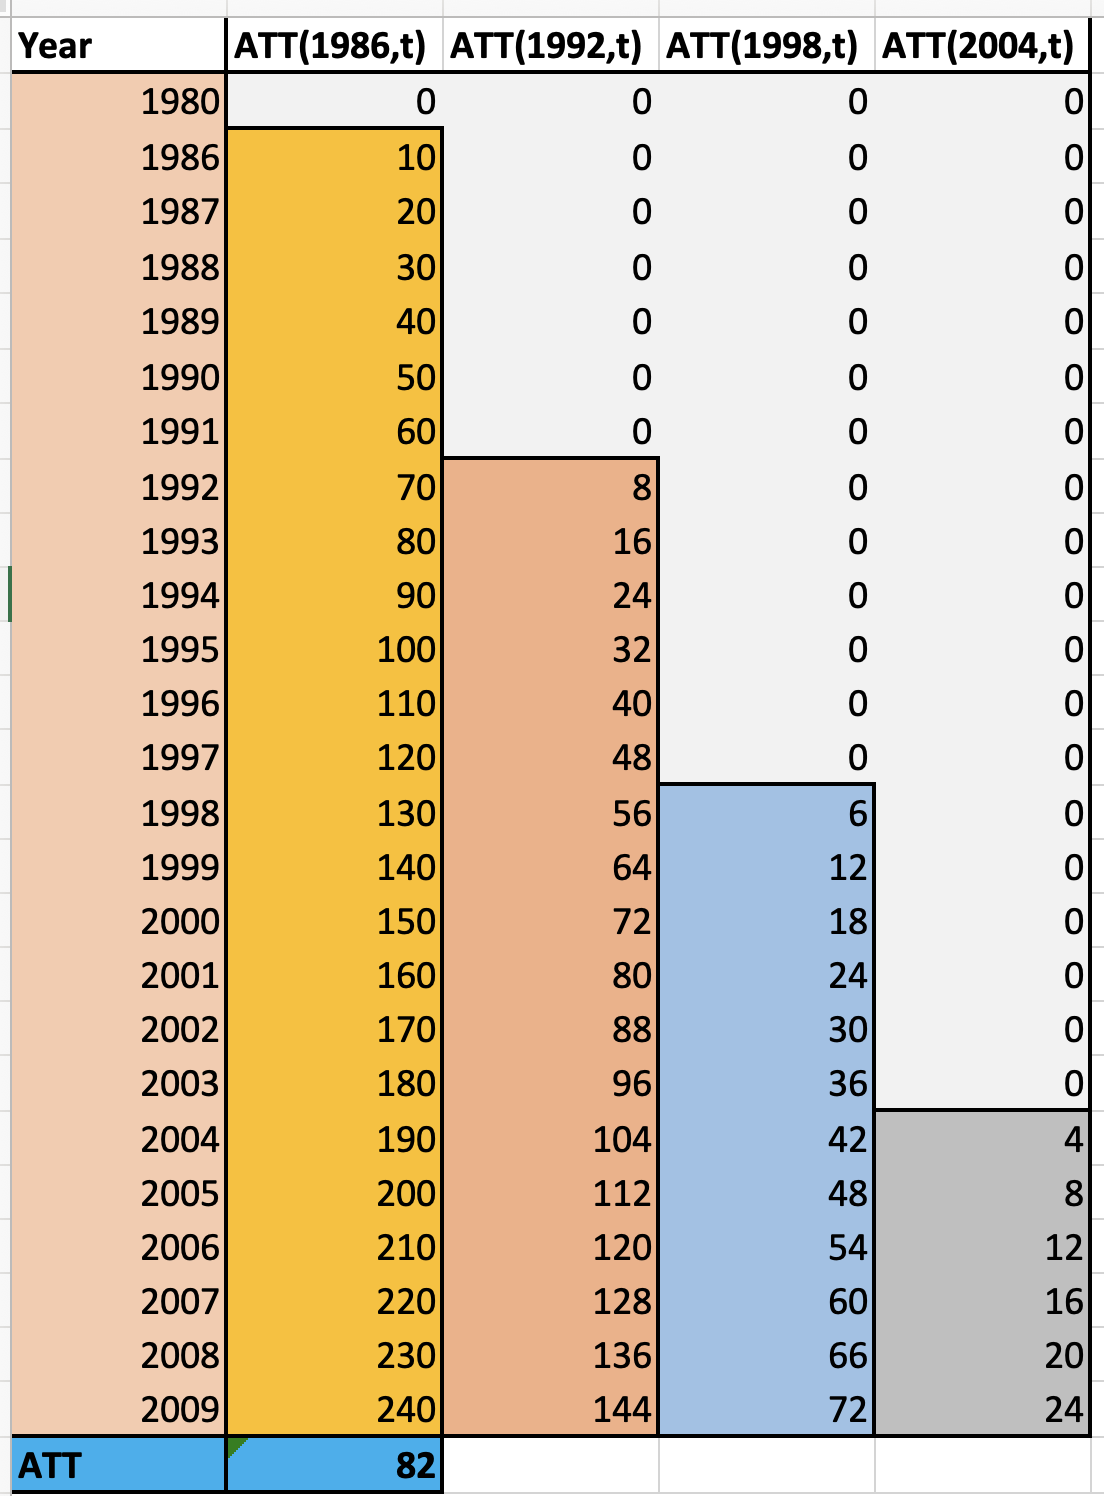
\includegraphics[height=6.5cm, width=5.5cm]{./lecture_includes/baker_attgt}
           \column{0.48\linewidth}
		\begin{itemize}
\item Heterogenous treatment effects across time and across groups
\item Cells are called ``group-time ATT'' (Callaway and Sant'anna 2020) or ``cohort ATT'' (Sun and Abraham 2020)
\item ATT is weighted average of all cells and $+82$ with uniform weights $1/60$
		\end{itemize}
         \end{columns} 
    \end{frame}

\begin{frame}{Estimation}

\bigskip

Estimate the following equation using OLS:

$$Y_{ist} = \alpha_i + \gamma_t +\delta D_{it} + \varepsilon_{ist}$$


\begin{table}[htbp]\centering
\small
\caption{Estimating ATT with different models}
\begin{center}
\begin{tabular}{l*{5}{c}}
\hline
\multicolumn{1}{l}{\textbf{}}&
\multicolumn{1}{c}{\textbf{Truth}}&
\multicolumn{1}{c}{\textbf{(TWFE)}}&
\multicolumn{1}{c}{\textbf{(CS)}}&
\multicolumn{1}{c}{\textbf{(SA)}}&
\multicolumn{1}{c}{\textbf{(BJS)}}\\
\hline
$\widehat{ATT}$  & 82    & -6.69*** &&&\\
\hline
\end{tabular}
\end{center}
\end{table}

The sign flipped.  Why?  Because of \emph{extreme} dynamics (i.e., $- \Delta ATT$)

\end{frame}

\begin{frame}{Bacon decomposition}
\begin{table}[htbp]\centering
\small
\caption{Bacon Decomposition (TWFE $= -6.69$)}
\begin{center}
\begin{tabular}{l*{5}{c}}
\hline
\multicolumn{1}{l}{\textbf{DD Comparison}}&
\multicolumn{1}{l}{\textbf{Weight}}&
\multicolumn{1}{l}{\textbf{Avg DD Est}}\\
\hline
Earlier T vs. Later C  &     0.500   &       51.800 \\
Later T vs. Earlier C   &    0.500    &     -65.180 \\
\midrule
T $=$ Treatment; C$ =$ Comparison \\
$(0.5*51.8) + (0.5*-65.180) = -6.69$ \\
\hline
\end{tabular}
\end{center}
\end{table}

\bigskip

While large weight on the ``late to early 2x2'' is \emph{suggestive} of an issue, these would appear even if we had constant treatment effects

\end{frame}





\subsection{CS}



\begin{frame}{Callaway and Sant'Anna 2020}

CS is a DiD model used for estimating ATT parameters under differential timing and conditional parallel trends


\begin{figure}
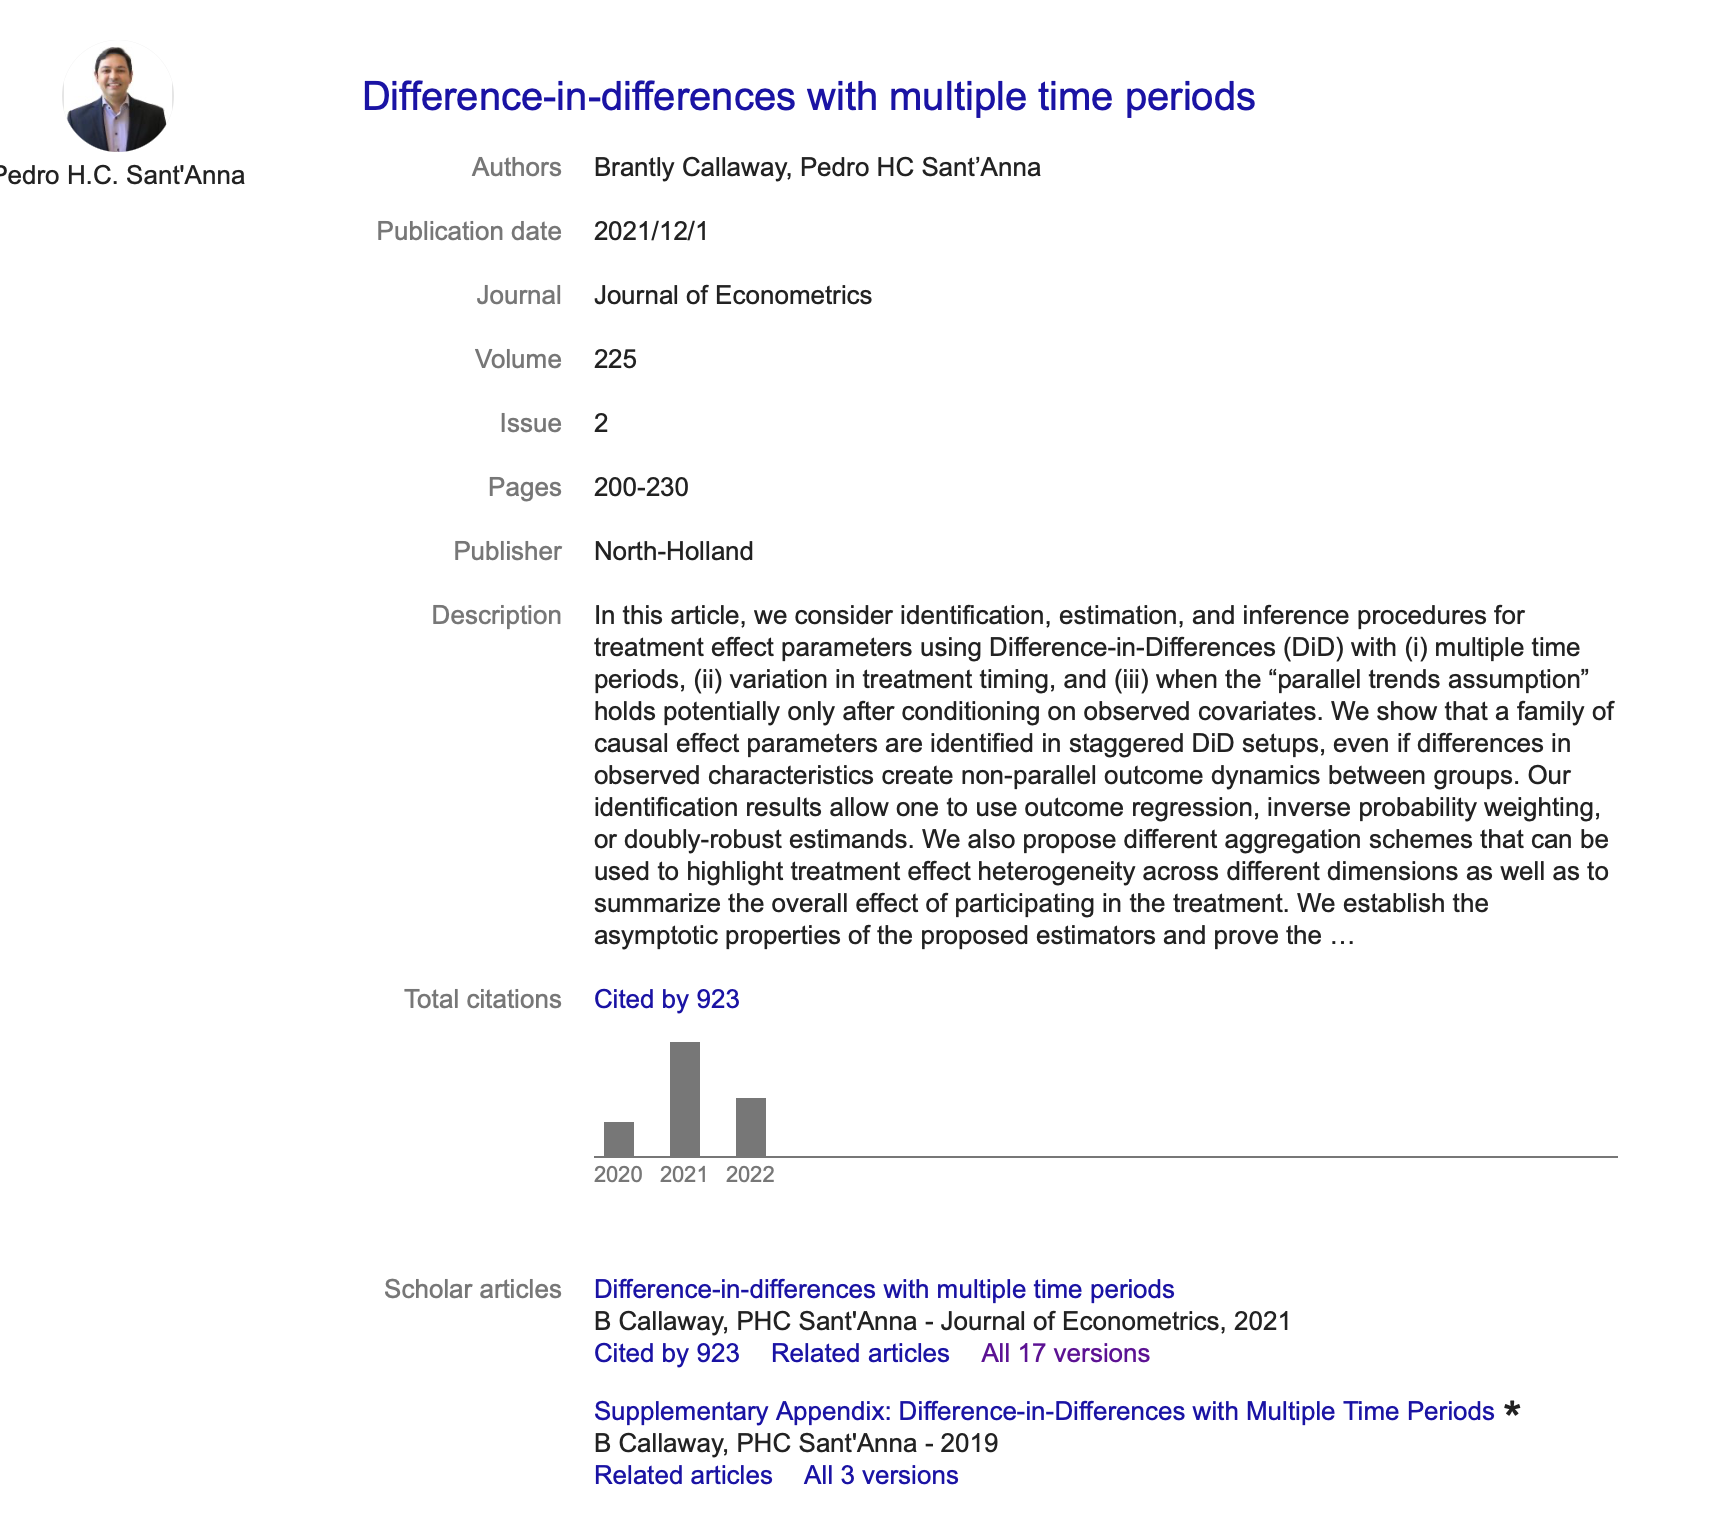
\includegraphics[scale=0.25]{./lecture_includes/pedro_cites}
\end{figure}

\end{frame}


\begin{frame}{When is CS used}

Just some examples of when you'd want to consider it:
\begin{enumerate}
\item When treatment effects differ depending on when it was adopted
\item When treatment effects change over time
\item When shortrun treatment effects more pronounced than longrun effects
\item When treatment effect dynamics differ if people are first treated in a recession relative to expansion years
\end{enumerate}

\bigskip

In other words -- CS is used to identity and aggregate heterogenous treatment effects

\end{frame}






\begin{frame}{Group-time ATT}
       \begin{columns}
          \column{0.38\linewidth}
             \centering
             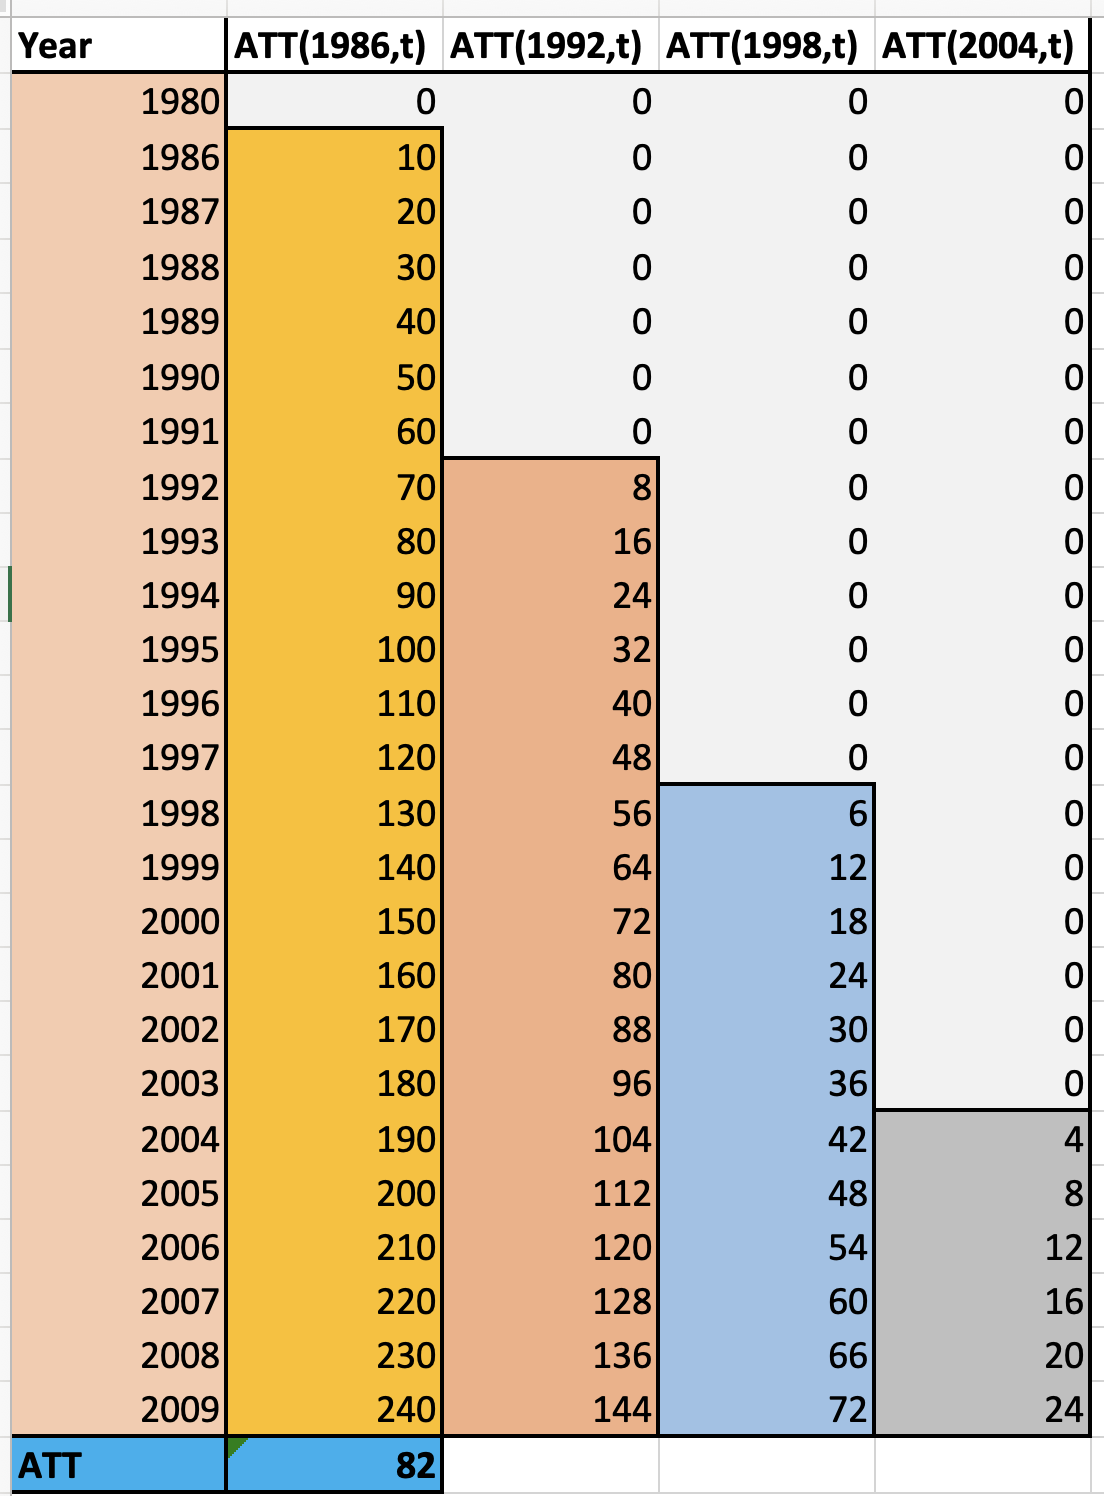
\includegraphics[height=6.5cm, width=5.5cm]{./lecture_includes/baker_attgt}
           \column{0.38\linewidth}
            Each cell contains that group's ATT(g,t)
\begin{eqnarray*}
ATT(g,t) = E[Y_t^1 - Y_t^0 | G_g=1]
\end{eqnarray*}CS identifies all feasible ATT(g,t)
         \end{columns} 
    \end{frame}




\begin{frame}{Group-time ATT}

Group-time ATT is the ATT for a specific group and time
\begin{itemize}
\item Groups are basically cohorts of units treated at the same time
\item Group-time ATT estimates are simple (weighted) differences in means
\item Does not directly restrict heterogeneity with respect to observed covariates, timing or the evolution of treatment effects over time
\item Allows us ways to choose our aggregations
\item Inference is the bootstrap
\end{itemize}

\end{frame}



\begin{frame}{Notation}

\begin{itemize}
\item $T$ periods going from $t=1, \dots, T$
\item Units are either treated ($D_t=1$) or untreated ($D_t=0$) but once treated cannot revert to untreated state
\item $G_g$ signifies a group and is binary.  Equals one if individual units are treated at time period $t$.
\item $C$ is also binary and indicates a control group unit equalling one if ``never treated'' (can be relaxed though to ``not yet treated'')
	\begin{itemize}
	\item Recall the problem with TWFE on using treatment units as controls
	\end{itemize}
\item Generalized propensity score enters into the estimator as a weight: $$\widehat{p(X)} = Pr(G_g=1 | X,G_g+C=1)$$
\end{itemize}

\end{frame}

\begin{frame}{Assumptions}

Assumption 1: Sampling is iid (panel data) \\
\bigskip
Assumption 2: Conditional parallel trends (for either never treated or not yet treated) \\
\begin{eqnarray*}
E[Y_t^0 - Y_{t-1}^0 | X,G_g=1] = [Y_t^0 - Y_{t-1}^0 | X,C=1] 
\end{eqnarray*}
\bigskip
Assumption 3: Irreversible treatment \\
Assumption 4: Common support (propensity score) \\
\bigskip
Assumption 5: Limited treatment anticipation (i.e., $ATT=0$ at baseline $g-1$)

\end{frame}

\begin{frame}{CS Estimator (the IPW version)}

\begin{eqnarray*}
ATT(g,t) = E \bigg [ \bigg ( \frac{G_g}{E[G_g]} - \frac{ \frac{\hat{p}(X)C}{1-\hat{p}(X)}}{E \bigg [ \frac{\hat{p}(X)C}{1-\hat{p}(X)} \bigg ]} \bigg ) (Y_t - Y_{g-1} ) \bigg ) \bigg ]
\end{eqnarray*}

This is the inverse probability weighting estimator.  Alternatively, there is an outcome regression approach and a doubly robust. Sant'Anna recommends DR. Notice how CS doesn't use already-treated as controls through subsetting the data with $C$
\end{frame}



\begin{frame}{Staggered adoption (i.e., universal coverage)}


\begin{proof}{\textbf{Remark 1:}}
In some applications, eventually all units are treated, implying that $C$ is never equal to one. In such cases one can consider the ``not yet treated'' ($D_t = 0$) as a control group instead of
the ``never treated?'' ($C = 1$).
\end{proof}

\end{frame}

\begin{frame}{Aggregated vs single year/group ATT}

\begin{itemize}
\item The method they propose is really just identifying very narrow ATT per group time.
\item But we are often interested in  more aggregate parameters, like the ATT across all groups and all times
\item They present two alternative methods for building ``interesting parameters'' 
\item Inference from a bootstrap
\end{itemize}


\end{frame}



\begin{frame}{Group-time ATT }
             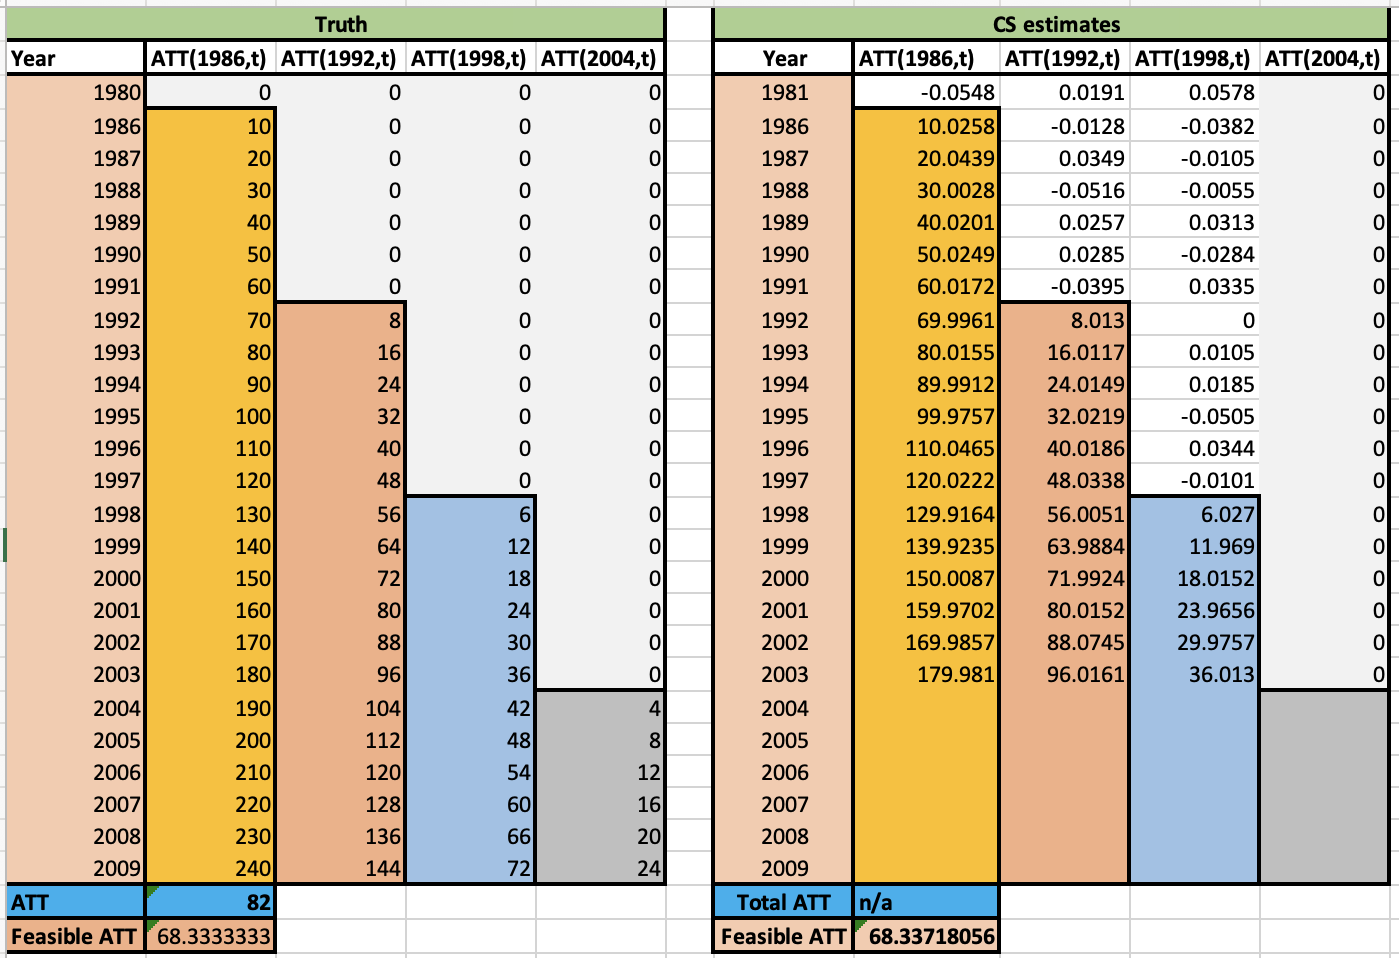
\includegraphics[scale=0.45]{./lecture_includes/baker_attgt_cs}

Question: Why didn't CS estimate all ATT(g,t)? What is ``feasible ATT''?

\end{frame}

\begin{frame}{Reporting results}
\begin{table}[htbp]\centering
\small
\caption{Estimating ATT using only pre-2004 data}
\begin{center}
\begin{tabular}{l*{5}{c}}
\hline
\multicolumn{1}{l}{\textbf{}}&
\multicolumn{1}{c}{\textbf{(Truth)}}&
\multicolumn{1}{c}{\textbf{(TWFE)}}&
\multicolumn{1}{c}{\textbf{(CS)}}&
\multicolumn{1}{c}{\textbf{(SA)}}&
\multicolumn{1}{c}{\textbf{(BJS)}}\\
\hline
$\widehat{Feasible\ ATT}$  & 68.33    & 26.81 *** & 68.34*** &&\\
\hline
\end{tabular}
\end{center}
\end{table}

TWFE is no longer negative, interestingly, once we eliminate the last group (giving us a never-treated group), but is still suffering from attenuation bias. 

\end{frame}



\subsection{SA}

\begin{frame}{Event study and differential timing}

\begin{itemize}
\item Event studies with one treatment group and one untreated group were relatively straightforward
\item Interact treatment group with calendar date to get a series of leads and lags
\item But when there are more than one treatment group, specification challenges emerge
\end{itemize}

\end{frame}


\begin{frame}{Differential timing complicates plotting sample averages}

\begin{itemize}
\item New Jersey treated in late 1992, New York in late 1993, Pennsylvania never treated
\item What years are each state's post-treatment?
	\begin{itemize}
	\item New Jersey: post-1992
	\item New York: post-1993
	\item Pennsylvania: ?
	\end{itemize}
\item How did people go about event studies then?

\end{itemize}

\end{frame}

\begin{frame}{Early efforts at event studies}

	\begin{figure}
	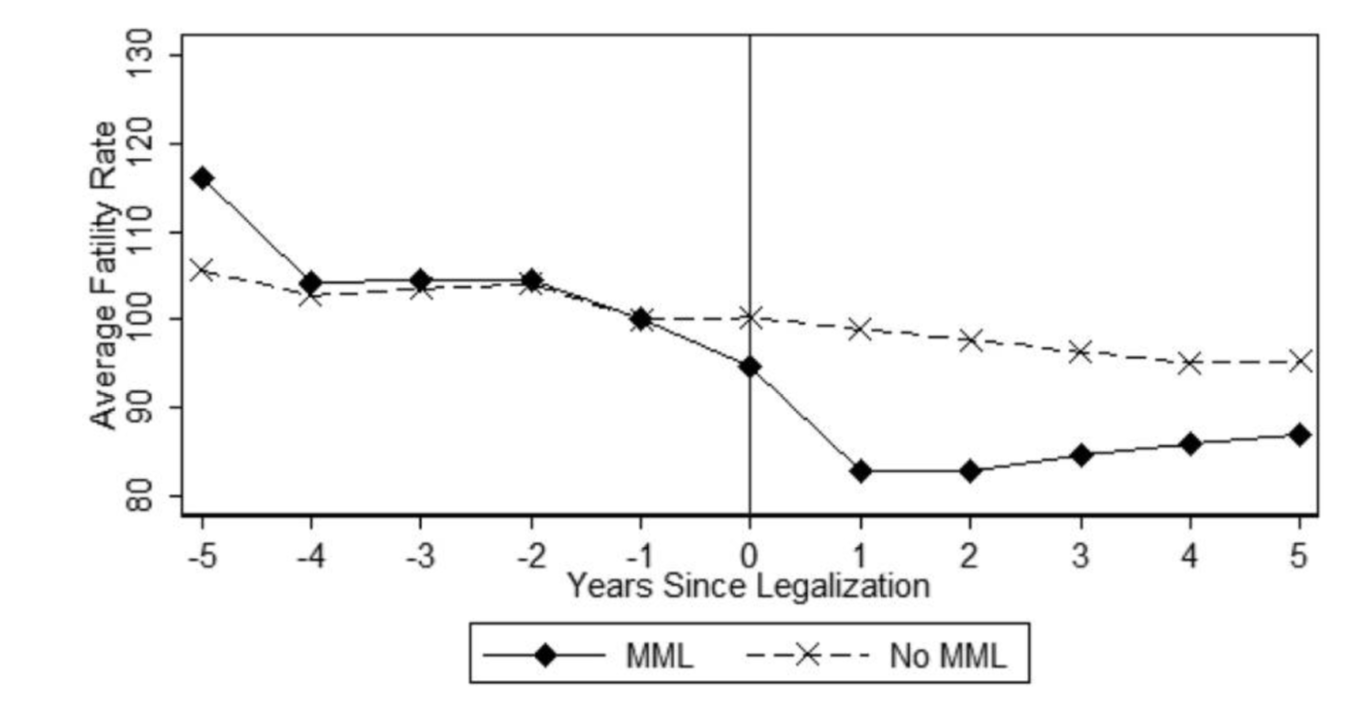
\includegraphics[scale=0.25]{./lecture_includes/mml_eventstudy.png}
	\caption{Anderson, et al. (2013) display of raw traffic fatality rates for re-centered treatment states and control states with randomized treatment dates}
	\end{figure}

\end{frame}

\begin{frame}{Replicated from a project of mine}

	\begin{figure}
	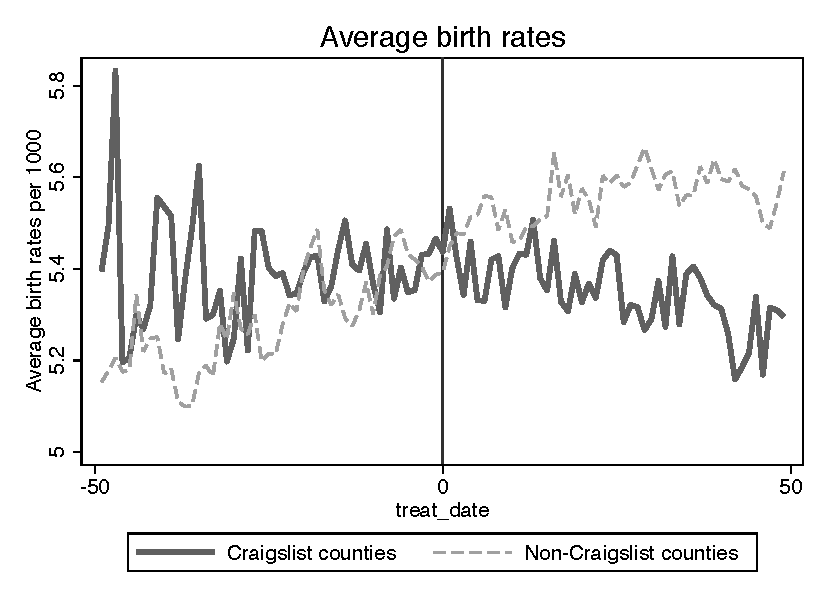
\includegraphics[scale=0.5]{./lecture_includes/dd.pdf}
	\caption{From one of my studies. Looks decent right?}
	\end{figure}

\end{frame}

\begin{frame}{Canonical event study specification with TWFE}


\begin{eqnarray*}
Y_{i,t} = \alpha_i + \delta_t + \sum_{g \in G} \mu_g1\{t-E_i \in g \} + \varepsilon_{i,t}
\end{eqnarray*}

\bigskip

Coefficient $\mu_g$ on a dummy measuring the number of years prior to or after that unit was treated.  This model, it turned out, suffered from model misspecification. 

\end{frame}

\begin{frame}[plain]
	\begin{figure}
	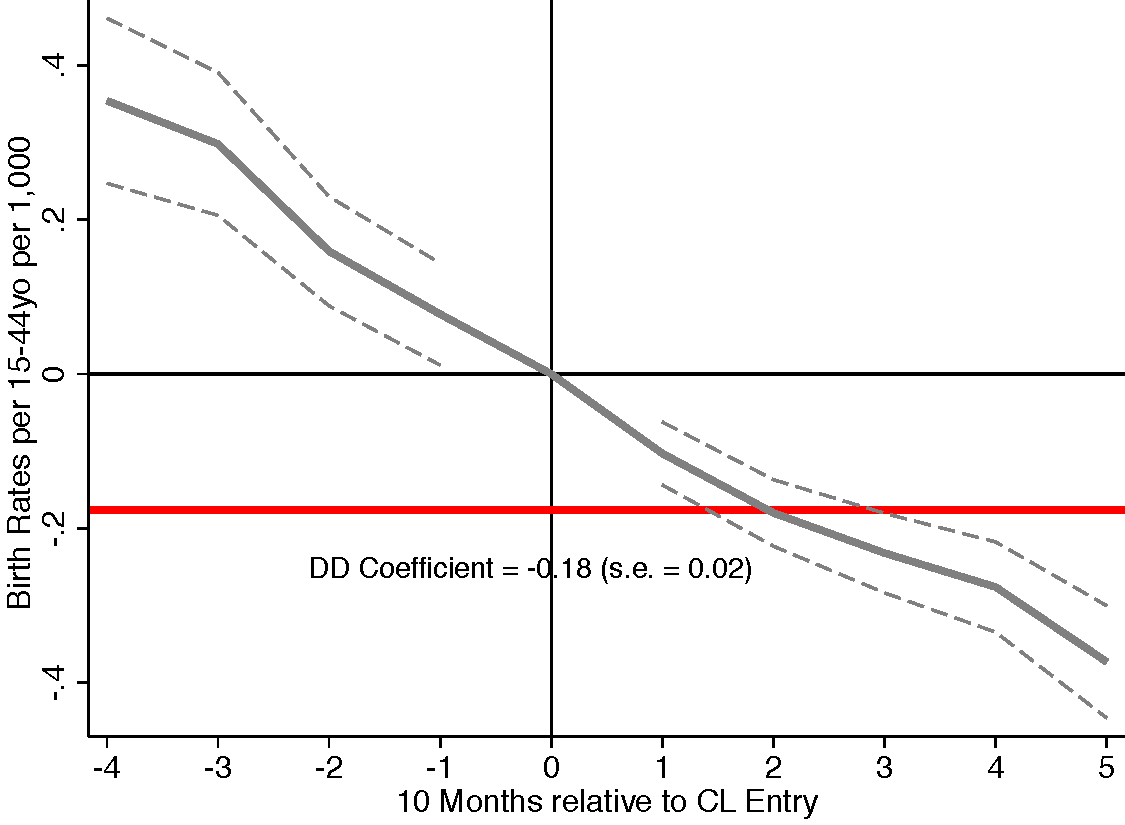
\includegraphics[scale=0.5]{./lecture_includes/br1544.pdf}
	\end{figure}
	
Same data as a couple slides ago, leads don't look good, so I abandoned the project. 
	
\end{frame}





\begin{frame}{Sun and Abraham 2020}

\begin{itemize}
\item Now that we know about the biases of the constant treatment effect model estimated with TWFE, let's revisit event studies under differential timing
\item Goodman-Bacon (2022) focused on decomposition of TWFE to show bias under differential timing
\item Callaway and Sant'anna (2020) presents alternative estimator that yields unbiased estimates of group-time ATTs which can be aggregated or put into event study plots
\item Sun and Abraham (SA) is like a combination of the two papers
\end{itemize}

\end{frame}

\begin{frame}{Background}

Sophie Sun was a grad student at MIT when she and Sarah Abraham came up with the idea of this paper. Listen to her briefly recount that story.

\url{https://youtu.be/bd8uSGsv32w?t=161}

\end{frame}


\begin{frame}{Summarizing (cont.)}

	\begin{enumerate}
	\item SA is a decomposition of the population regression coefficient on event study leads and lags with differential timing estimated with TWFE
	\item They show that the population regression coefficient is ``contaminated'' by information from other leads and lags
	\item SA presents an alternative estimator that is a version of CS only using the ``last cohort'' as the treatment group (not the not-yet-treated)
	\end{enumerate}

\end{frame}

\begin{frame}{Summarizing (cont.)}

\begin{itemize}
\item Under homogenous treatment profiles, weights sum to zero and``cancel out'' the treatment effects from other periods 
\item Under treatment effect heterogeneity, they do not cancel out and leads and lags are biased
\item They present a 3-step TWFE based alternative estimator which addresses the problems that they find
\end{itemize}

\end{frame}


\begin{frame}{Some notation and terms}

\begin{itemize}
\item As people often \textbf{bin} the data, we allow a lead or lag $l$ to appear in bin $g$ so sometimes they use $g$ instead of $l$ or $l \in g$
\item Building block is the ``cohort-specific ATT'' or $CATT_{e,l}$ -- same as ATT(g,t)
\item Our goal is to estimate $CATT_{e,l}$ with population regression coefficient $\mu_l$
\item They focus on irreversible treatment where treatment status is non-decreasing sequence of zeroes and ones
\end{itemize}

\end{frame}



\begin{frame}{Difficult notation (cont.)}

\begin{itemize}
\item The $\infty$ symbol is used to either describe the group ($E_i=\infty$) or the potential outcome ($Y^{\infty}$)
\item $Y^{\infty}_{i,t}$ is is the potential outcome for unit $i$ if it had never received treatment (versus received it later), also called the baseline outcome
\item Other counterfactuals are possible -- maybe unit $i$ isn't ``never treated'' but treated later in counterfactual
\end{itemize}
\end{frame}

\begin{frame}{More difficult notation (cont.)}

\begin{itemize}
\item Treatment effects are the difference between the observed outcome relative to the never-treated counterfactual outcome: $Y_{i,t} - Y^{\infty}_{i,t}$
\item We can take the average of treatment effects at a given relative time period across units first treated at time $E_i=e$ (same cohort) which is what we mean by $CATT_{e,l}$
\item Doesn't use $t$ index time (``calendar time''), rather uses $l$ which is time until or time after treatment date $e$ (``relative time'')
\item Think of it as ${l}=$year - treatment date
\end{itemize}

\end{frame}

\begin{frame}{Relative vs calendar event time}


\begin{figure}
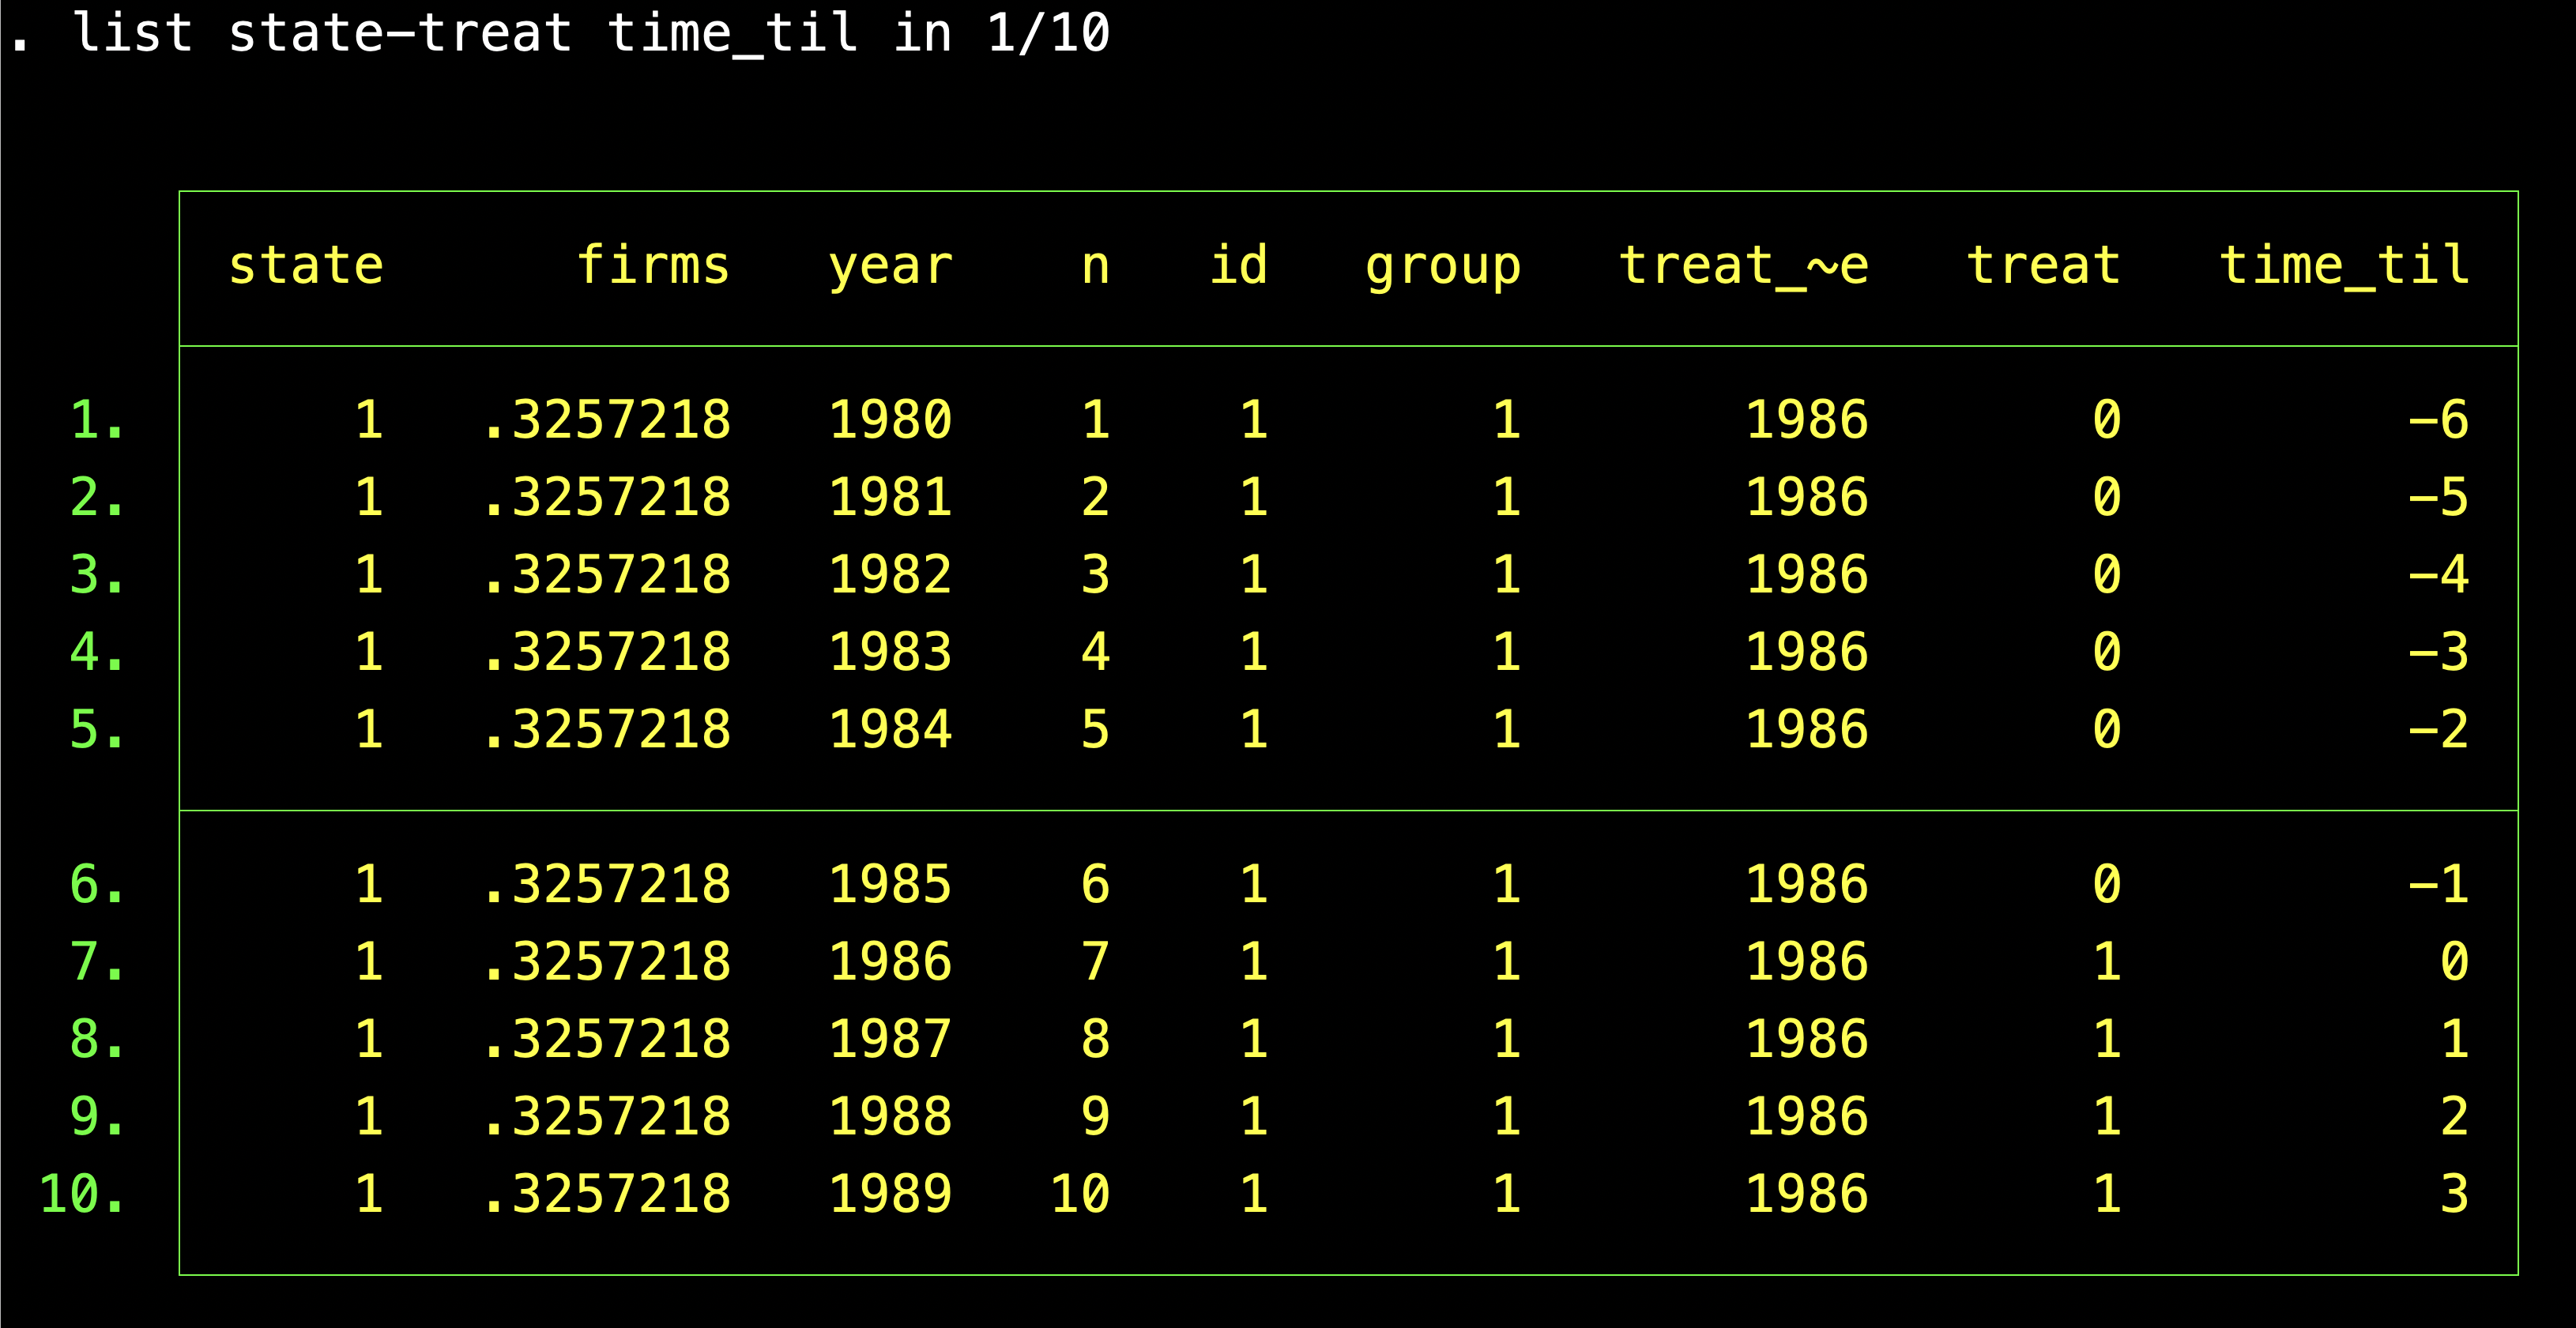
\includegraphics[scale=0.2]{./lecture_includes/timetil}
\end{figure}

\end{frame}


\begin{frame}{Definition 1}

\textbf{Definition 1:} The cohort-specific ATT $l$ periods from initial treatment date $e$ is:

\begin{eqnarray*}
CATT_{e,l} = E[Y_{i,e+l} - Y^{\infty}_{i,e+l} | E_i=e]
\end{eqnarray*}

\bigskip

Fill out the second part of the Group-time ATT exercise together.

\end{frame}

\begin{frame}{TWFE assumptions}

\begin{itemize}
\item For consistent estimates of the coefficient leads and lags using TWFE model, we need three assumptions
\item For SA and CS, we only need two
\item Let's look then at the three
\end{itemize}

\end{frame}


\begin{frame}{Assumption 1: Parallel trends}

\textbf{Assumption 1: Parallel trends in baseline outcomes}: $E[Y^{\infty}_{i,t} - Y^{\infty}_{i,s} | E_i = e ]$ is the same for all $e \in supp(E_i)$ and for all $s$, $t$ and is equal to $E[Y^{\infty}_{i,t} - Y^{\infty}_{i,s} ]$

\bigskip

Lead and lag coefficients are DiD equations but once we invoke parallel trends they can become causal parameters.  This reminds us again how crucial it is to have  appropriate controls

\end{frame}


\begin{frame}{Assumption 2: No anticipation}

\textbf{Assumption 2: No anticipator behavior in pre-treatment periods}: There is a set of pre-treatment periods such that $E[Y_{i,e+l}^e - Y_{i,e+l}^{\infty} | E_i = e]=0$ for all possible leads.

\bigskip

Essentially means that pre-treatment, the causal effect is zero.  Most plausible if no one sees the treatment coming, but even if they see it coming, they may not be able to make adjustments that affect outcomes

\end{frame}


\begin{frame}{Assumption 3: Homogeneity}

\textbf{Assumption 3: Treatment effect profile homogeneity}: For each relative time period $l$, the $CATT_{e,l}$ doesn't depend on the cohort and is equal to $CATT_l$. 


\end{frame}

\begin{frame}{Treatment effect heterogeneity}

\begin{itemize}
\item Assumption 3 is violated when different cohorts experience different paths of treatment effects
\item Cohorts may differ in their covariates which affect how they respond to treatment (e.g., if treatment effects vary with age, and there is variation in age across units first treated at different times, then there will be heterogeneous treatment effects)
\item Doesn't rule out parallel trends
\end{itemize}

\end{frame}

\begin{frame}{Event study model}

\begin{eqnarray*}
Y_{i,t} = \alpha_i + \delta_t + \sum_{g \in G} \mu_g1\{t-E_i \in g \} + \varepsilon_{i,t}
\end{eqnarray*}

\bigskip

We are interested in the properties of $\mu_g$ under differential timing as well as whether there are any never-treated units

\end{frame}



\begin{frame}[plain, shrink=20]
\begin{center}
\textbf{Interpreting $\widehat{\mu_g}$ under no to all assumptions}
\end{center}

\textbf{Proposition 1 (no assumptions):} The population regression coefficient on relative period bin $g$ is a linear combination of differences in trends from its own relative period $l \in g$, from relative periods $l \in g'$ of other bins $g' \neq g$, and from relative periods excluded from the specification (e.g., trimming). 

\begin{eqnarray*}
\mu_g &=& \underbrace{\sum_{l \in g} \sum_{e} w^g_{e,l} \big ( E[Y_{i,e+l} - Y^{\infty}_{i,0} | E_i = e] - E[Y^{\infty}_{i,e+l} - Y^{\infty}_{i,0}] \big )}_{\mathclap{\text{Targets}}} \\
&+& \underbrace{\sum_{g' \neq g} \sum_{l \in g'} \sum_e w^g_{e,l} \big ( E[Y_{i,e+l} - Y^{\infty}_{i,0} | E_i=e] - E[Y^{\infty}_{i,e+l} - Y^{\infty}_{i,0}] \big )}_{\mathclap{\text{Contamination from other leads and lags}}} \\
&+&  \underbrace{\sum_{l \in g^{excl}} \sum_{e} w^g_{e,l} \big ( E[Y_{i,e+l} - Y^{\infty}_{i,0} | E_i=e] - E[Y^{\infty}_{i,e+l} - Y^{\infty}_{i,0}] \big )}_{\mathclap{\text{Contamination from dropped periods}}} 
\end{eqnarray*}

\bigskip


\end{frame}

\begin{frame}{Weight ($w^g_{e,l}$) summation cheat sheet}

\begin{enumerate}
\item For relative periods of $\mu_g$ own $l \in g$, $\sum_{l \in g}\sum_ew^g_{e,l}=1$
\item For relative periods belonging to some other bin $l\in g'$ and $g' \neq g$, t $\sum_{l \in g'}\sum_ew^g_{e,l} = 0$
\item For relative periods not included in $G$, $\sum_{l \in g^{excl}} \sum_e w^g_{e,l} = -1$
\end{enumerate}

\end{frame}




\begin{frame}{Estimating the weights}

Regress $D^l_{i,t} \times 1\{E_i=e \}$ on:

\begin{enumerate}
\item all bin indicators included in the main TWFE regression, 
\item $\{ 1\{ t-E_i \in g \} \}_{g \in G}$(i.e., leads and lags) and 
\item the unit and time fixed effects
\end{enumerate}

\end{frame}


\begin{frame}{Still biased under parallel trends}

\textbf{Proposition 2}: Under the parallel trends only, the population regression coefficient on the indicator for relative period bing $g$ is a linear combination of $CATT_{e,l \in g}$ as well as $CATT_{d,l'}$ from other relative periods $l' \notin g$ with the same weights stated in Proposition 1:

\begin{eqnarray*}
\mu_g &=& \underbrace{\sum_{l \in g} \sum_e w^g_{e,l} CATT_{e,l}}_{\mathclap{\text{Desirable}}} \\
&& + \underbrace{\sum_{g' \neq g, g' \in G} \sum_{l' \in g'} \sum_e w^g_{e,l'}  CATT_{e,l'}}_{\mathclap{\text{Bias from other specified bins}}} \\
&&+ \underbrace{\sum_{l' \in g^{excl}} \sum_e w^g_{e,l'} CATT_{e,l'}}_{\mathclap{\text{Bias from dropped relative time indicators}}}
\end{eqnarray*}



\end{frame}


\begin{frame}{Still biased under parallel trends and no anticipation}

\textbf{Proposition 3}: If parallel trends holds and no anticipation holds for all $l<0$ (i.e., no anticipatory behavior pre-treatment), then the population regression coefficient $\mu_g$ for $g$ is a linear combination of post-treatment $CATT_{e,l'}$ for all $l' \geq 0$.

\begin{eqnarray*}
\mu_g &=& \sum_{l' \in g, l' \geq 0} \sum_e w^g_{e,l'} CATT_{e,l'} \\
&&+ \sum_{g' \neq g,g' \in G} \sum_{l' \in g', l' \geq 0} \sum_e w^g_{e,l'} CATT_{e,l'} \\
&&+ \sum_{l' \in g^{excl},l' \geq 0} \sum_e w^g_{w,l'} CATT_{e,l'}
\end{eqnarray*}

\end{frame}

\begin{frame}{Proposition 3 comment}

Notice how once we impose zero pre-treatment treatment effects, those terms are gone (i.e., no $l \in g, l<0$).  But the second term remains unless we impose treatment effect homogeneity (homogeneity causes terms due to weights summing to zero to cancel out). Thus $\mu_g$ may be non-zero for pre-treatment periods \emph{even though parallel trends hold in the pre period.}

\end{frame}

\begin{frame}{Proposition 4}

\textbf{Proposition 4}: If parallel trends and treatment effect homogeneity, then $CATT_{e,l}=ATT_l$ is constant across $e$ for a given $l$, and the population regression coefficient $\mu_g$ is equal to a linear combination of $ATT_{l \in g}$, as well as $ATT_{l' \notin g}$ from other relative periods

\begin{eqnarray*}
\mu_g &=& \sum_{l \in g} w^g_l ATT_l \\
&&+ \sum_{g' \neq g} \sum_{l' \in g'} w^g_{l'} ATT_{l'} \\
&&+ \sum_{l' \in g^{excl}} w^g_{l'}ATT_{l'}
\end{eqnarray*}


\end{frame}

\begin{frame}{Simple example}


Balanced panel $T=2$ with cohorts $E_i \in \{1,2 \}$. For illustrative purposes, we will include bins $\{-2,0\}$ in our calculations but drop $\{-1,1\}$. 


\end{frame}

\begin{frame}{Simple example}

\begin{eqnarray*}
\mu_{-2} &=& \underbrace{CATT_{2,-2}}_{\mathclap{\text{own period}}} + \underbrace{\frac{1}{2}CATT_{1,0} - \frac{1}{2} CATT_{2,0}}_{\mathclap{\text{other included bins}}} \\
&&+ \underbrace{ \frac{1}{2} CATT_{1,1} - CATT_{1,-1} - \frac{1}{2} CATT_{2,-1} }_{\mathclap{\text{Excluded bins}}}
\end{eqnarray*}

\begin{itemize}
\item Parallel trends gets us to all of the $CATT$
\item No anticipation makes $CATT=0$ for all $l<0$ (all $l<0$ cancel out)
\item Homogeneity cancels second and third terms
\item Still leaves $\frac{1}{2} CATT_{1,1}$ -- you chose  to exclude a group with a treatment effect
\end{itemize}Lesson: drop the relative time indicators on the left, not things on the right, bc lagged effects will contaminate through the excluded bins


\end{frame}


\begin{frame}{Robust event study estimation}


\begin{itemize}
\item All the robust estimators under differential timing have solutions and they all skip over forbidden contrasts. 
\item Sun and Abraham (2020) propose a 3-step interacted weighted estimator (IW) using last treated group as control group
\item Callaway and Sant'anna (2020) estimate group-time ATT which can be a weighted average over relative time periods too but uses ``not-yet-treated'' as control
\end{itemize}

\end{frame}




\begin{frame}{Interaction-weighted estimator}

\begin{itemize}
\item \textbf{Step one}: Do this DD regression and hold on to $\widehat{\delta}_{e,l}$
\end{itemize}

\begin{eqnarray*}
Y_{i,t} = \alpha_i + \lambda_t + \sum_{e \notin C} \sum_{l \neq -1} \delta_{e,l} \big (1 \{ E_i = e \} \cdot D_{i,t}^l \big ) + \varepsilon_{i,t}
\end{eqnarray*}


\bigskip

Can use never-treated or last-treated cohort. Drop always treated. The $\delta_{e,l}$ is a DD estimator for $CATT_{e,l}$ with particular choices for pre-period and cohort controls

\end{frame}


\begin{frame}{Interaction-weighted estimator}

\begin{itemize}
\item \textbf{Step two}: Estimate weights using sample shares of each cohort in the relevant periods:
\end{itemize}

\begin{eqnarray*}
Pr(E_i=e|E_i \in [-l,T-l])
\end{eqnarray*}

\end{frame}

\begin{frame}{Interaction-weighted estimator}

\begin{itemize}
\item \textbf{Step three}: Take a weighted average of estimates for $CATT_{e,l}$ from Step 1 with weight estimates from step 2
\end{itemize}


\begin{eqnarray*}
\widehat{v}_g = \frac{1}{|g|} \sum_{l \in g} \sum_e \widehat{\delta}_{e,l} \widehat{Pr} \{ E_i=e | E_i \in [-l,T-l]\}
\end{eqnarray*}


\end{frame}

\begin{frame}{Consistency and Inference}


\begin{itemize}
\item Under parallel trends and no anticipation, $\widehat{\delta}_{e,l}$ is consistent, and sample shares are also consistent estimators for population shares. 
\item Thus IV estimator is consistent for a weighted average of $CATT_{e,l}$ with weights equal to the share of each cohort in the relevant period(s).
\item They show that each IW estimator is asymptotically normal and derive its asymptotic variance. Doesn't rely on bootstrap like CS.
\end{itemize}

\end{frame}

\begin{frame}{DD Estimator of CATT}

\textbf{Definition 2}: DD estimator with pre-period $s$ and control cohorts $C$ estimates $CATT_{e,l}$ as:

\begin{eqnarray*}
\widehat{\delta_{e,l}} = \frac{ E_N \big [ \big ( Y_{i, e+l} - Y_{i,s} \big ) \times 1\{E_i=e\} \big ]}{E_N[1 \{E_i=e\} ]} - \frac{E_N \big [ \big ( Y_{i,e+l} \times 1 \{E_i \in C \} ]}{E_N [1 \{ E_i \in C \}]}
\end{eqnarray*}


\textbf{Proposition 5}: If parallel trends and no anticipation both hold for all pre-periods, then the DD estimator using any pre-period and non-empty control cohorts (never-treated or not-yet-treated) is an unbiased estimate for $CATT_{e,l}$

\end{frame}

\begin{frame}{Software}

\begin{itemize}
\item \textbf{Stata}: eventstudyinteract (can be installed from ssc)
\item \textbf{R}: fixest with subab() option (see \url{https://lrberge.github.io/fixest/reference/sunab.html/})
\end{itemize}


\end{frame}


\begin{frame}{Reporting results}
\begin{table}[htbp]\centering
\small
\caption{Estimating ATT}
\begin{center}
\begin{tabular}{l*{5}{c}}
\hline
\multicolumn{1}{l}{\textbf{}}&
\multicolumn{1}{c}{\textbf{(Truth)}}&
\multicolumn{1}{c}{\textbf{(TWFE)}}&
\multicolumn{1}{c}{\textbf{(CS)}}&
\multicolumn{1}{c}{\textbf{(SA)}}&
\multicolumn{1}{c}{\textbf{(BJS)}}\\
\hline
$\widehat{Feasible\ ATT}$  & 68.33    & 26.81*** & 68.34*** & 68.33***&\\
\hline
\end{tabular}
\end{center}
\end{table}

\end{frame}

\begin{frame}{Computing relative event time leads and lags }
             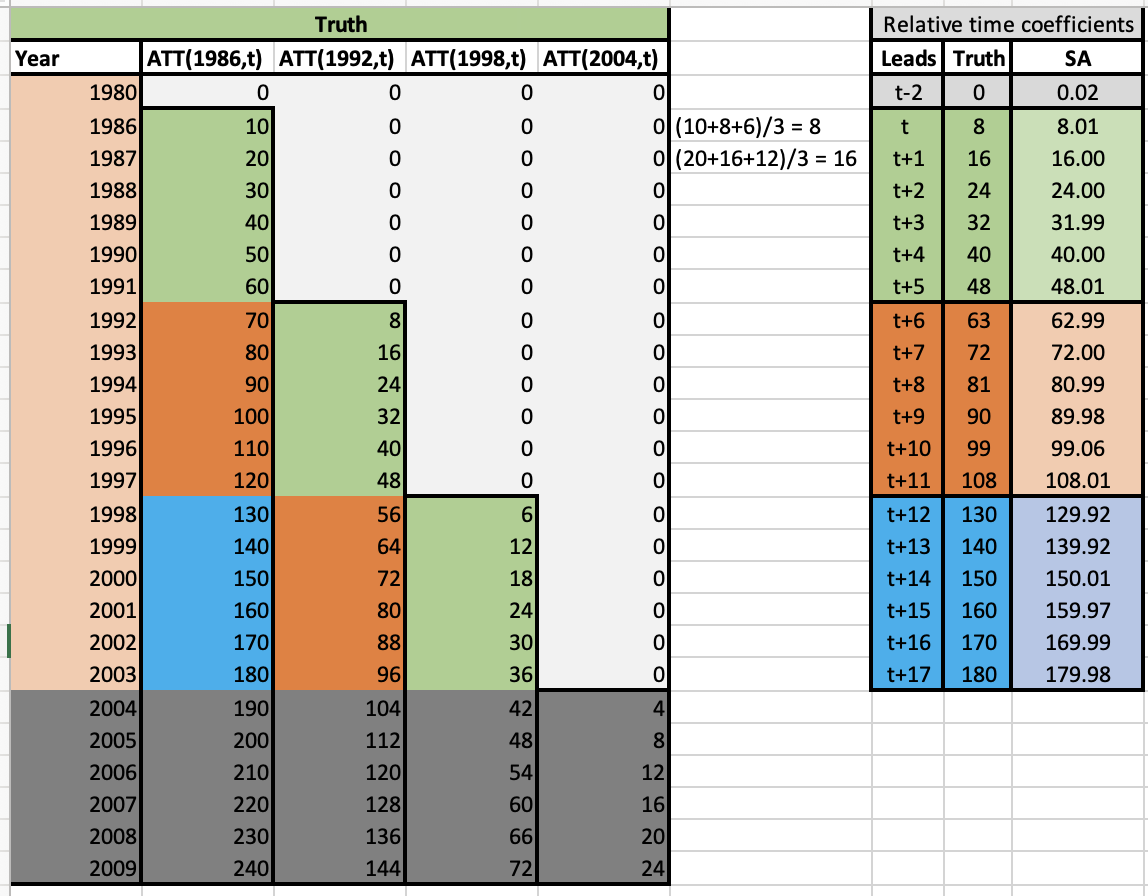
\includegraphics[scale=0.45]{./lecture_includes/sa_leads}

Two things to notice: (1) there only 17 lags with robust models but will be 24 with TWFE; (2) changing colors mean what?

\end{frame}

\begin{frame}{Comparing TWFE and SA }

\begin{figure}
\begin{center}
             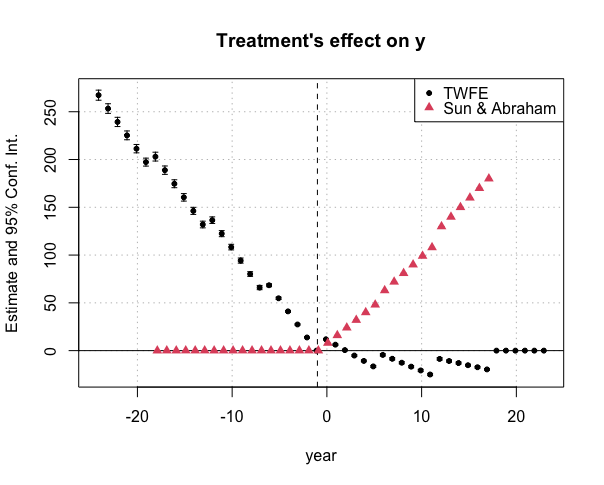
\includegraphics[scale=0.4]{./lecture_includes/twfe_sa_event}
\end{center}
\end{figure}

Question: why is TWFE \emph{falling} pre-treatment?  Why is SA rising, but jagged, post-treatment?

\end{frame}
\subsection{Imputation}

\begin{frame}{Causal inference is always imputing counterfactuals}

\begin{quote}
``At some level, all methods for causal inference can be viewed as imputation methods, although some more explicitly than others.'' -- Imbens and Rubin (2015)
\end{quote}

\end{frame}


\begin{frame}{Causal inference involves imputation}

\begin{itemize}
\item Causal inference is a missing data problem -- we are missing counterfactuals
\item And recall that estimating the ATT necessarily involved correctly imputing the counterfactual using parallel trends
\item OLS, therefore, is \emph{implicitly} imputing counterfactuals for estimating the ATT
\end{itemize}

\end{frame}


\begin{frame}{Imputation methods}

All recent working papers

\bigskip

	\begin{enumerate}
	\item \textbf{2SDiD} (Gardner 2021) -- imputes $Y^0$ using estimated fixed effects from the $D=0$ units, residualizing into $\widehat{Y}$, regressing new $\widehat{Y}$ using GMM
	\item \textbf{Robust efficient imputation} (Borusyak, et al. 2021) -- very similar to 2SDID in that you impute $Y^0$ using $D=0$ sample and estimated fixed effects 
	\item \textbf{Mundlak} (Wooldridge 2022) -- TWFE with saturated interactions, is equivalent to the above two
	\end{enumerate}

There is also Athey, et al. (2020) matrix completion with nuclear norm regularization but since it it does not depend on parallel trends (rather it nests synthetic control), it is not a DiD method

\end{frame}


\begin{frame}{Steps for BJS}

Target parameter is individual treatment effect, $\delta_i$

\begin{enumerate}
\item Estimate expected potential outcomes using OLS and only the untreated observations (this is similar to Gardner 2021)
\item Then calculate $\widehat{\delta}_{it} = Y_{it}^1 - \widehat{Y}_{it}^0$
\item Then estimate target parameters as weighted sums$$\widehat{\delta}_W = \sum_{it}w_{it}\widehat{\delta}_{it}$$
\end{enumerate}

\end{frame}


\begin{frame}{Why is this working?}

\begin{itemize}
\item Because we can obtain consistent estimates of the fixed effects, we can extrapolate to the counterfactual units for all $Y(0)_{it}$ that were treated
\item This is the same type of trick we see with Heckman, et al. (1997) as well as Gardner (2021) 
\item As it is still OLS, it's computationally fast and flexible to unit-trends, triple diff, covariates and so forth (with caveats about time-varying covariates requiring more assumptions)
\item Wooldridge shows the Mundak estimator maps onto BJS robust model
\end{itemize}

\end{frame}


\begin{frame}{Reporting results}
\begin{table}[htbp]\centering
\small
\caption{Estimating ATT}
\begin{center}
\begin{tabular}{l*{5}{c}}
\hline
\multicolumn{1}{l}{\textbf{}}&
\multicolumn{1}{c}{\textbf{(Truth)}}&
\multicolumn{1}{c}{\textbf{(TWFE)}}&
\multicolumn{1}{c}{\textbf{(CS)}}&
\multicolumn{1}{c}{\textbf{(SA)}}&
\multicolumn{1}{c}{\textbf{(BJS)}}\\
\hline
$\widehat{Feasible\ ATT}$  & 68.33    & 26.81*** & 68.34*** & 68.33***& 68.33***\\
\hline
\end{tabular}
\end{center}
\end{table}

\end{frame}

\begin{frame}{Software}

\begin{enumerate}
\item Callaway and Sant'anna (2020)
	\begin{itemize}
	\item \textbf{Stata}: csdid
	\item \textbf{R}: did
	\end{itemize}
\item Sun and Abraham (2020)
	\begin{itemize}
	\item \textbf{Stata}: eventstudyinteract 
	\item \textbf{R}: fixest with subab() option 
	\end{itemize}
\item Borusyak, et al. (2022) 
	\begin{itemize}
	\item \textbf{Stata}: dd\_imputation
	\item \textbf{R}: didimputation
	\end{itemize}
\item Gardner (2021)
	\begin{itemize}
	\item \textbf{Stata}: did2s
	\item \textbf{R}: did2s
	\end{itemize}
\end{enumerate}

\end{frame}

\section{Concluding Remarks}


\begin{frame}{Encouragement}
	\begin{itemize}
	\item Models give identical results for ``strong parallel trends'' types of assumptions (though confidence intervals differ)
	\item Choose estimator based on which parallel trend assumption you feel most comfortable with is my suggestion
	\item Encourage you to use authors' own packages as they have the incentive to fix bugs and maintain it
	\end{itemize}
\end{frame}






\end{document}



\subsection{dCH}

\begin{frame}{de Chaisemartin and D'Haultfoeulle 2020}

de Chaisemartin and D'Haultfouelle 2020 (dCdH) is different from the other papers in several ways
	\begin{itemize}
	\item Like SA, it's a diagnosis and a cure
	\item TWFE decomposition shows coefficient a weighted average of underlying treatment effects, but weights can be negative negating causal interpretation
	\item Propose a solution for both static and dynamic specification which does not use already treated as controls
	\item Treatment can turn on and off
	\end{itemize}

\end{frame}


\begin{frame}{Comment on Bacon}

\begin{itemize}
\item Recall the Bacon decomposition -- TWFE coefficients are decomposed into weighted average of all underlying 2x2s. Weights were non-negative and summed to one.
\item But this decomposition was more a numerical decomposition -- what exactly adds up to equal the TWFE coefficient using the data we observe?
\item Bacon's decomposition is not ``theoretical'' -- not in the way that other decompositions are. He is just explaining what OLS ``does'' when it calculates $\widehat{\delta}$
\item Just explains what comparisons OLS is using to calculate the TWFE coefficient -- just peels back the curtain.
\end{itemize}

\end{frame}

\begin{frame}{Causal effects}

\begin{itemize}
\item dCdH impose causal assumptions and try a different decomposition strategy
\item Uses as its building block the unit-specific treatment effects
\item This is hopefully going to help us better understand where these negative weights are coming from
\item Note that their model is very general in that the treatment is reversible (meaning you can turn it on and off)
\end{itemize}

\end{frame}

\begin{frame}{Terms}

\begin{itemize}
\item Target parameter: $$\Delta^g_{i,t} = Y^1_{i,t} - Y^\infty_{i,t}$$ but where the treatment is in time period $g$. Notice --it's not the ATT (it's $i$ individual treatment effect)
\item TWFE terms. Define the error term as $\varepsilon_{i,t}$: $$D_{i,t} = \alpha_i + \alpha_t + \varepsilon_{i,t}$$
\item Weights: $$w_{i,t} = \frac{\varepsilon_{i,t}}{\frac{1}{N^T} \sum_{i,t:D_{i,t}=1} \varepsilon_{i,t}}$$Basically divide the error by the average of the error for all treated units. 
\end{itemize}

\end{frame}

\begin{frame}{Assumptions}

\begin{block}{Strong unconditional PT}
Assume that for every time period $t$ and every group $g,g'$, $$E[Y^\infty_t - Y^\infty_{t-1}|G=g] = E[Y^\infty_t - Y^\infty_{t-1}|G=g'] $$
\end{block}Assume parallel trends for every unit in every cohort in every time period.

\end{frame}

\begin{frame}{dCdH Theorem}

\begin{block}{Theorem -- dCdH decomposition}
Assuming SUTVA, no anticipation and the strong PT, then let $\beta$ be the TWFE estimand associated with $$Y_{i,t} = \alpha_i + \alpha_t + \beta D_{i,t} + \varepsilon_{i,t}$$Then it follows that $$\beta = E \bigg [ \sum_{i,t:D_{i,t}=1} \frac{1}{N^T} w_{i,t} \cdot \Delta_{i,t}^g \bigg ] $$ where $\sum_{i,t:D_{i,t}=1} \frac{w_{i,t}}{N^T} = 1$ but $w_{i,t}$ can be negative
\end{block}So once you run that specification, $\beta$ is going to recover a non-convex average over all unit level treatment effects (weights can be negative). dCdH was the first I think.

\end{frame}


\begin{frame}{Negative weights}

\begin{itemize}
\item Very common now to hear about negative weights, and furthermore, that negative weights wipe out any causal interpretation, but why?
\item What if every unit treatment effect was positive, but some of the weights were negative?
\item It's possible it could flip the sign, but it would definitely at least pull the estimate away from the true effect
\item This is dangerous -- and it's caused by the forbidden contrasts (treated to already treated)
\end{itemize}

\end{frame}



\begin{frame}{Negative weights}

\begin{itemize}
\item Doesn't always pose a problem, but no proofs for this intuition known yet
\item A large number of never-treated seems to make this less an issue
\item Shrinking the spacing between treatment dates also can drive it down
\item But does that mean that TWFE works, and what does it mean to work?
\item TWFE still even when all the weights are positive the weighted average may not aggregate to what we think it does
\end{itemize}

\end{frame}

\begin{frame}{Weighting}

\begin{itemize}
\item The weights in OLS all come out of the model itself, \emph{not the economic question}
\item The economic question is ``what parameter do you want? What does it look like? Who is in it?''
\item And when you define the parameter up front, you've more or less defined the economic question you're asking
\item But OLS sort of ignores your question and just gives you what it wants
\end{itemize}

\end{frame}

\begin{frame}{Weighting}

\begin{itemize}
\item What makes something a good vs a bad weight?
\item Not being negative is the absolute minimal requirement
\item But it's also not a good sign if you can't really explain the weights
\end{itemize}

\end{frame}

\begin{frame}{dCdH Solution}

\begin{itemize}
\item dCdH propose an alternative that doesn't have the problems of TWFE -- both avoiding negative weights and improving interpretability
\item Recall, their model can handle reversible treatments

\end{itemize}

\end{frame}



